\chapter{Tool demonstration for load-following and safety analysis: Molten 
Salt Breeder Reactor}
The previous chapter has shown that the \gls{TAP} \gls{MSR} is unaffected by
xenon poisoning during power variation because it has a relatively 
fast neutron energy spectrum. 
While long-term performance metrics such as fuel utilization would definitely 
benefit from online removal of poisonous fission products, the gas removal 
system is not necessary to ensure safe \gls{TAP} system operation during a
short-term power drop and restart transient. 
However, Chapter 5 clearly demonstrated a strong impact of the noble gas 
removal on the reactor neutronics during power adjustments. Thus, another 
liquid-fueled \gls{MSR} design with thermal spectrum (not epithermal like in 
the \gls{TAP} core) was considered to investigate the benefits of the 
online gas removal for load-following operation.	

This chapter presents fuel salt depletion analysis with SaltProc during a
short-term power transient to evaluate load-following capabilities of the 
graphite-moderated molten salt reactor design with a thermal neutron energy 
spectrum - \glsfirst{MSBR}. The details of the \gls{MSBR} design, the 
full-core Serpent model, and the results of long-term depletion simulation 
with SaltProc were described in Chapter 3. I simulated the load-following 
transient postulated in Section~\ref{sec:worst-load} using the methodology 
described in Chapter 5. 
To investigate the effect of noble gas removal efficiency on the 
load-following operation, I considered three various regimes of the gas 
removal system operation:
\begin{enumerate}[label=(\alph*), noitemsep, topsep=0pt]
	\item no gas removal ($\epsilon_{Xe}=0.0$);
	\item moderate gas removal efficiency ($\epsilon_{Xe}=0.536$);
	\item high gas removal efficiency ($\epsilon_{Xe}=0.915$).
\end{enumerate}
I then calculated a major safety and operational parameters for all three 
regimes at various moments of the transient to ensure that the critical 
safety margins are maintained. Finally, I compared the \gls{TAP} \gls{MSR} and 
\gls{MSBR} behavior during the postulated load-following transient.


\section{Depletion analysis results}
I used the methodology described previously in Chapter 5 for the \gls{MSBR} 
full-core depletion analysis with SaltProc v1.0 with a 30-minute depletion 
time step to capture rapid changes in reactivity. 
Equation~\ref{eq:time-xe-max} predicted the time after shutdown when 
$^{135}$Xe concentration peaks ($t^{max}_X$) in the range from 6.8h 
($\epsilon_{Xe}=0.0$, 30 years after startup) to 7.5h ($\epsilon_{Xe}=0.915$, 
\gls{BOL}). The $t^{max}_X$ for the \gls{MSBR} is longer than 
for the \gls{TAP} reactor (2.75h) due to a much more thermal neutron energy 
spectrum. To be consistent throughout different gas removal regimes while 
investigating load-following capabilities of the \gls{MSBR}, I selected a
following transient (power load profile) very similar to the transient chosen 
in Chapter 5:
\begin{enumerate}[label=(\alph*), noitemsep, topsep=0pt]
	\item operate on 100\% of \gls{HFP} to reach $^{135}$I/$^{135}$Xe 
	equilibrium (at 
	least 3 days from the startup);
	\item instantaneous power drop from 100\% to 0\%;
	\item shutdown for $t^{max}_X=7.5h$ to reach the $^{135}$Xe concentration 
	extremum;
	\item instant restart from 0\% to 100\% power level and operate on 100\% 
	for 5 hours.
\end{enumerate}


\subsection{Reactivity dynamics}
Figures~\ref{fig:msbr-lf-keff-evo} and \ref{fig:msbr-lf-rho-evo} show the 
effective multiplication factor and reactivity dynamics for the various gas 
removal efficiencies in the \gls{MSBR} during the transient, 
described earlier. For the no-removal case (Figure~\ref{fig:msbr-lf-keff-evo}, 
upper panel), the effective multiplication factor dropped after 
$t^{max}_X=7.5h$ by 1457 $pcm$ and 1035 $pcm$ at \gls{BOL} and after 15 years 
of full-power operation, respectively. Thus, the Equation~\ref{eq:time-xe-max} 
correctly predicted the moment when the xenon poisoning effect maximized in the
no-removal case ($\epsilon_{Xe}=0$).
After the power ramp-up from 0\% to 100\%, the effective multiplication factor 
returned to its initial value in about 3 hours. Notably, maximum 
negative reactivity insertion due to $^{135}$Xe buildup after the 
\gls{MSBR} shutdown is very similar to the \gls{PWR} (both at startup): 1457 
$pcm$ and 1500 $pcm$ \cite{rykhlevskii_impact_2019}, respectively. 
Additionally, the xenon poisoning effect diminished toward the \gls{EOL} 
because the $^{135}$Xe concentration peak is more significant for the softer 
thermal spectrum (the \gls{MSBR} spectrum becomes \emph{harder} during  
operation due to plutonium and other strong neutron absorbers accumulation in 
the fuel salt).
Finally, the effect of $^{135}$Xe poisoning is almost the same after 15 and 30 
years of operation because the fuel salt composition reaches its equilibrium 
after about 16 years of full-power operation (see 
Section~\ref{sec:ch3-msbr-fuel-comp}).

The middle and lower plots in Figure~\ref{fig:msbr-lf-rho-evo} show reactivity 
change during the \gls{MSBR} shutdown for 7.5 hours and following power ramp 
up to 100\% for moderate ($\epsilon_{Xe}=0.536$) and high 
($\epsilon_{Xe}=0.915$) removal efficiency, respectively. In contrast with 
no gas removal, reactivity dropped during the 30-minutes interval after 
shutdown by 161 $pcm$ and 189 $pcm$ for moderate and high removal efficiency, 
respectively.  Afterward, the reactivity boosts by 1494 $pcm$ and 2608 $pcm$ 
for $\epsilon_{Xe}=0.536$ and 0.915, respectively. Such reactivity change 
happens because the gas removal system extracted 53.6\% and 91.5\% of xenon 
mass at the end of the 30-minute depletion step. The more effective xenon 
removal leads to greater 
positive reactivity jump, as expected. Notably, the reactivity stabilizes at 
approximately $+2500$ $pcm$ level about 5 hours after the shutdown because 
the $^{135}$Xe loss due to its decay and online 
gas removal equalizes $^{135}$Xe gain from $^{135}$I decay.
Overall, the online gas removal from the fuel salt even with moderate 
efficiency is beneficial to the core neutronics and significantly reduces the 
xenon poisoning effect ($-161\pm10$ $pcm$ instead of $-1494\pm10$ $pcm$). 
Moreover, the very high removal efficiency ($\epsilon_{Xe}=0.915$) is 
unnecessary to significantly reduce the effect of xenon poisoning and enable 
the load-following capability of the \gls{MSBR}.
\begin{figure}[htbp!] % replace 't' with 'b' to 
	\centering
$\begin{array}{c}
	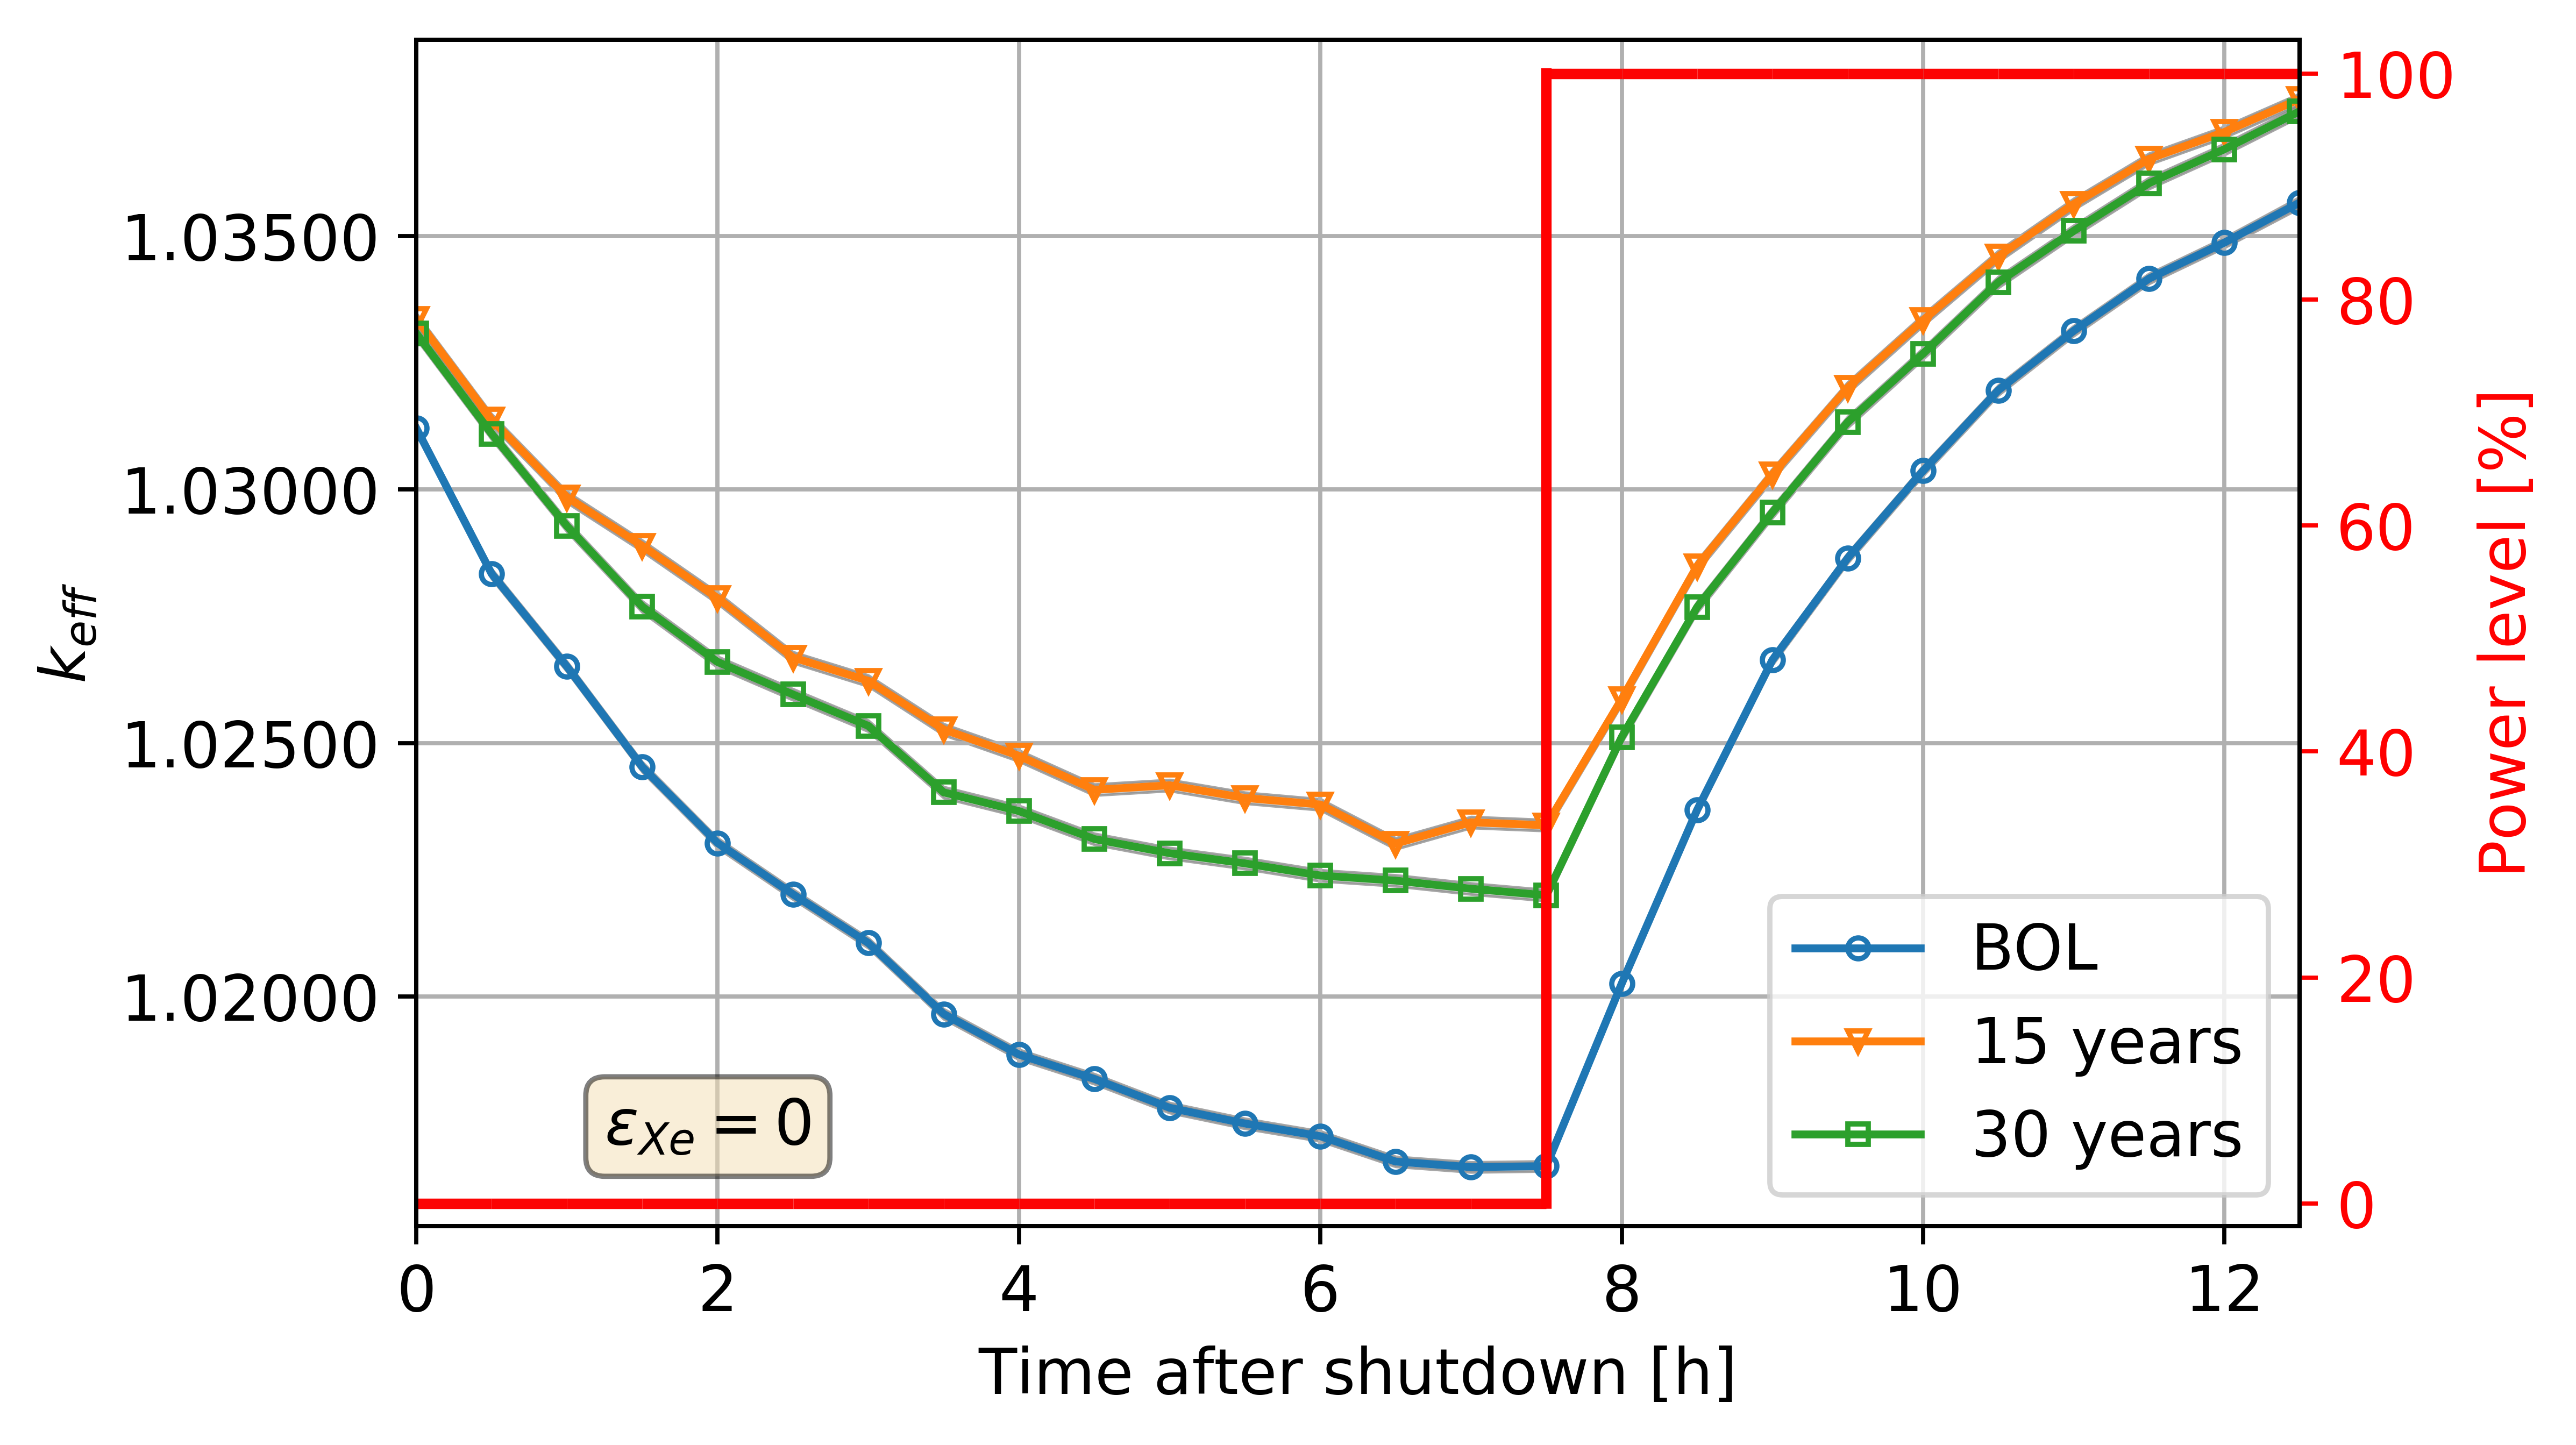
\includegraphics[width=0.92\textwidth]{ch6/kl1_keff.png}\vspace{-14mm}\\
	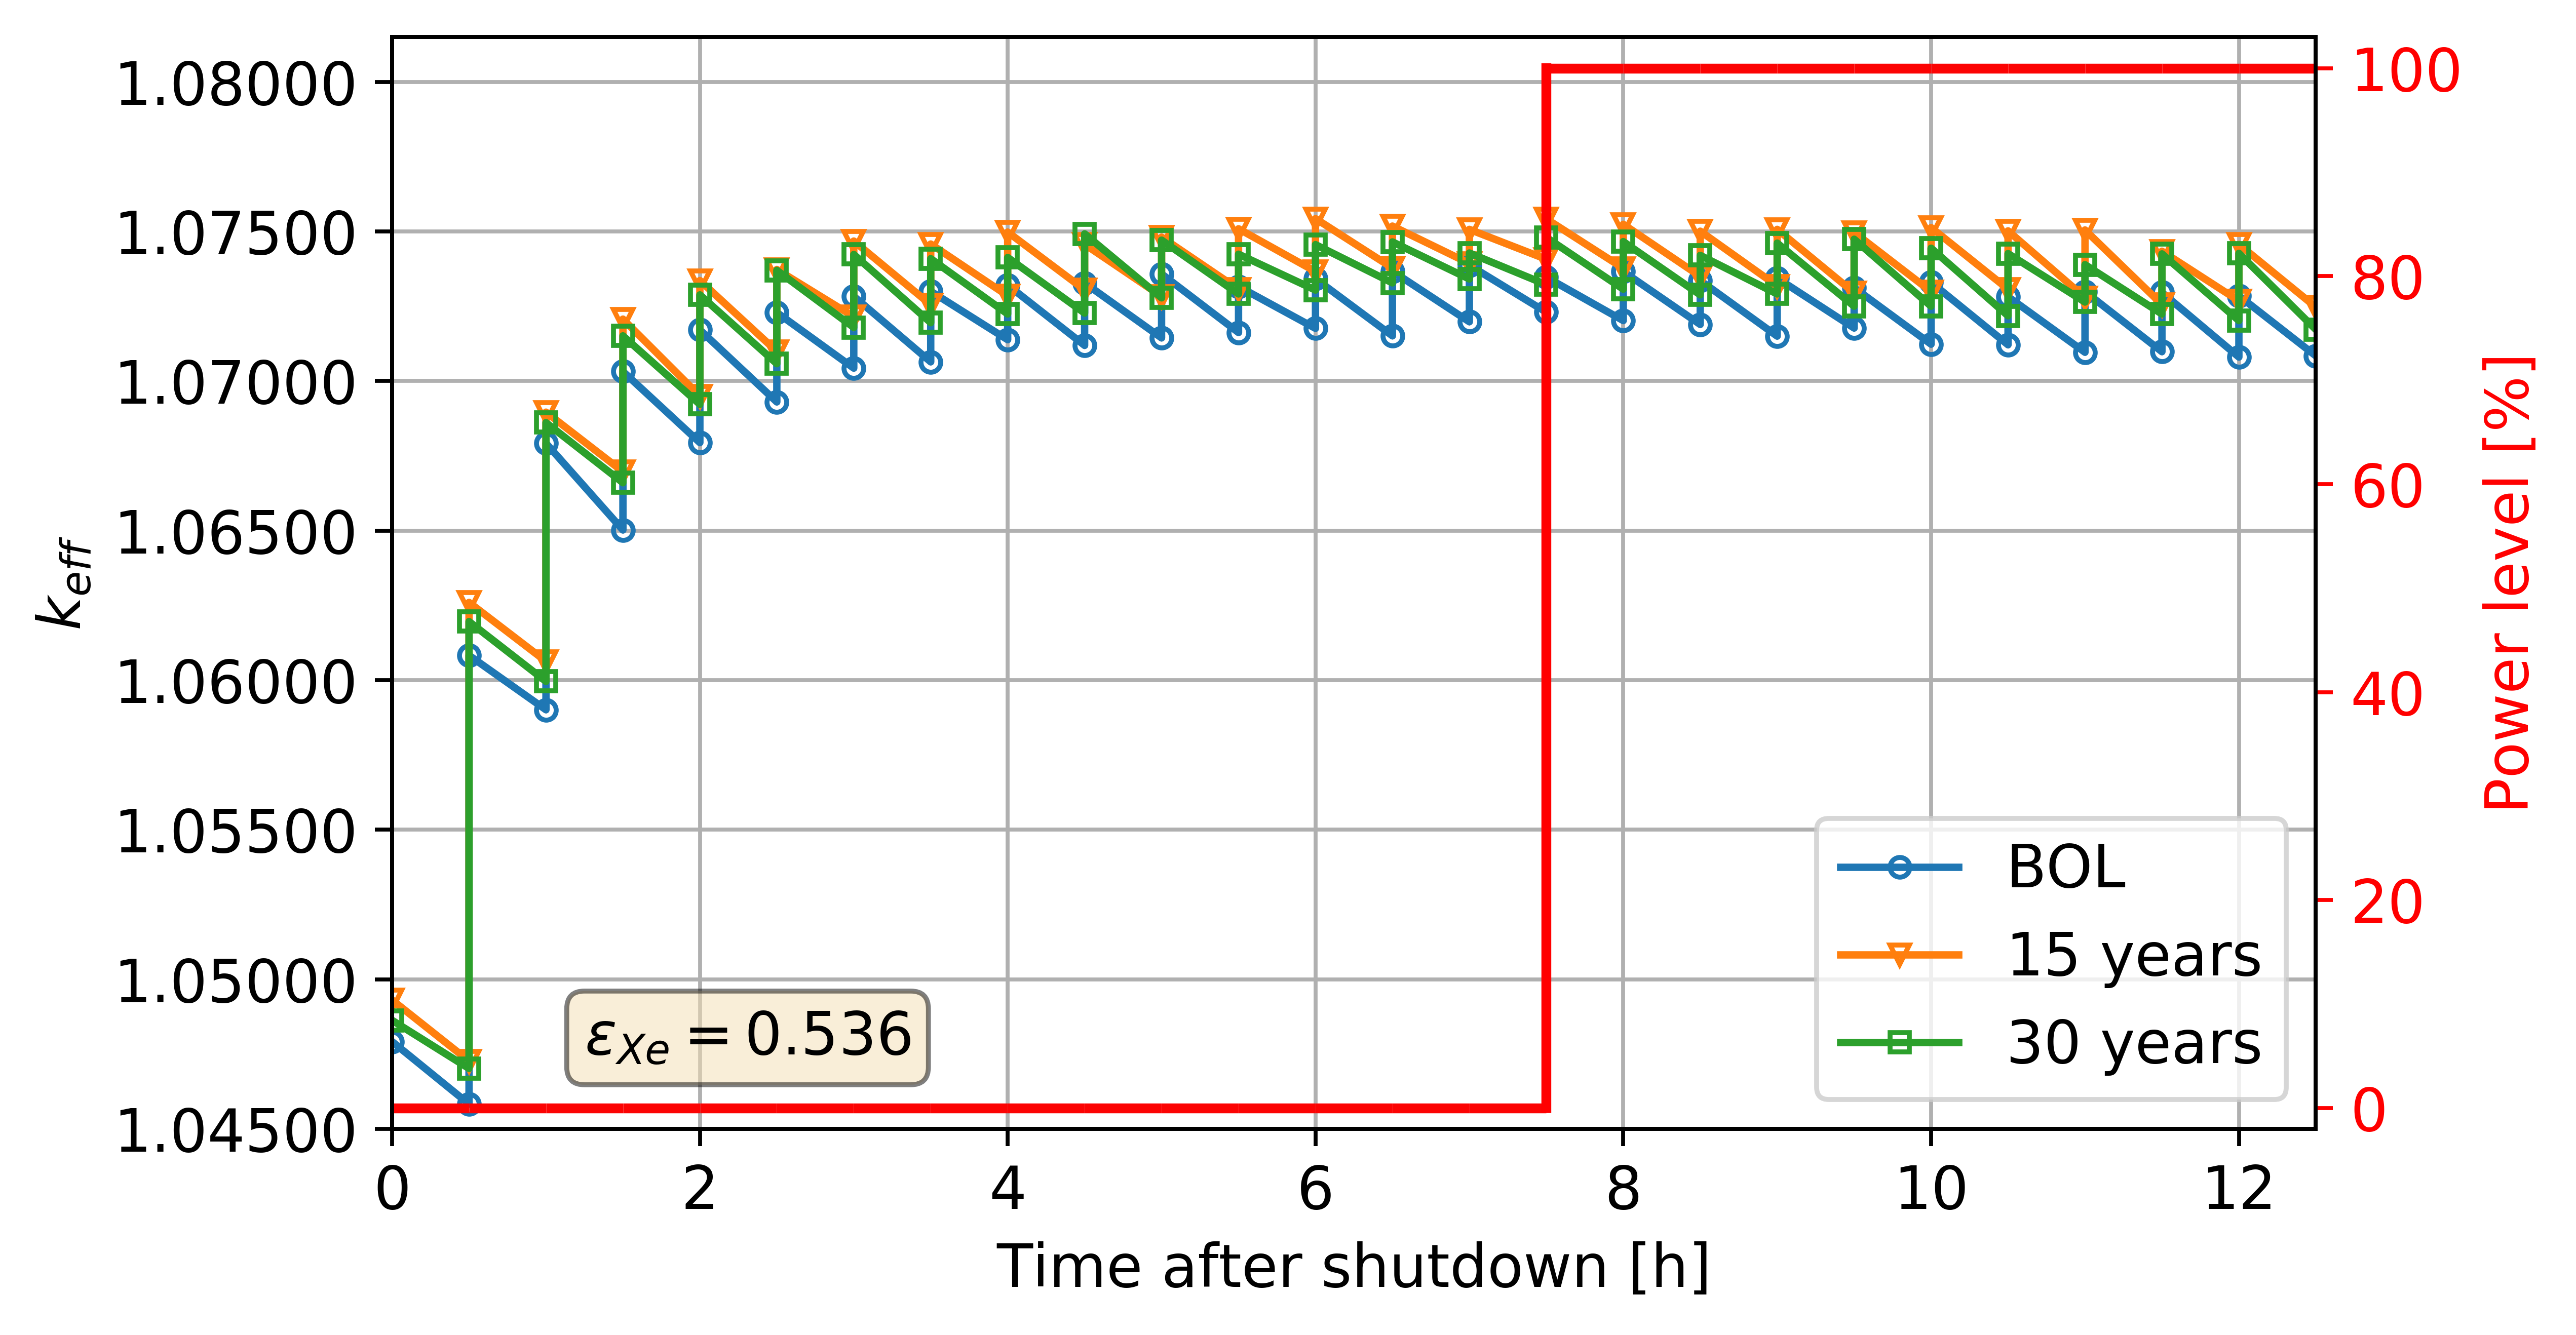
\includegraphics[width=0.905\textwidth]{ch6/kl25_keff.png}\vspace{-12mm}\\
	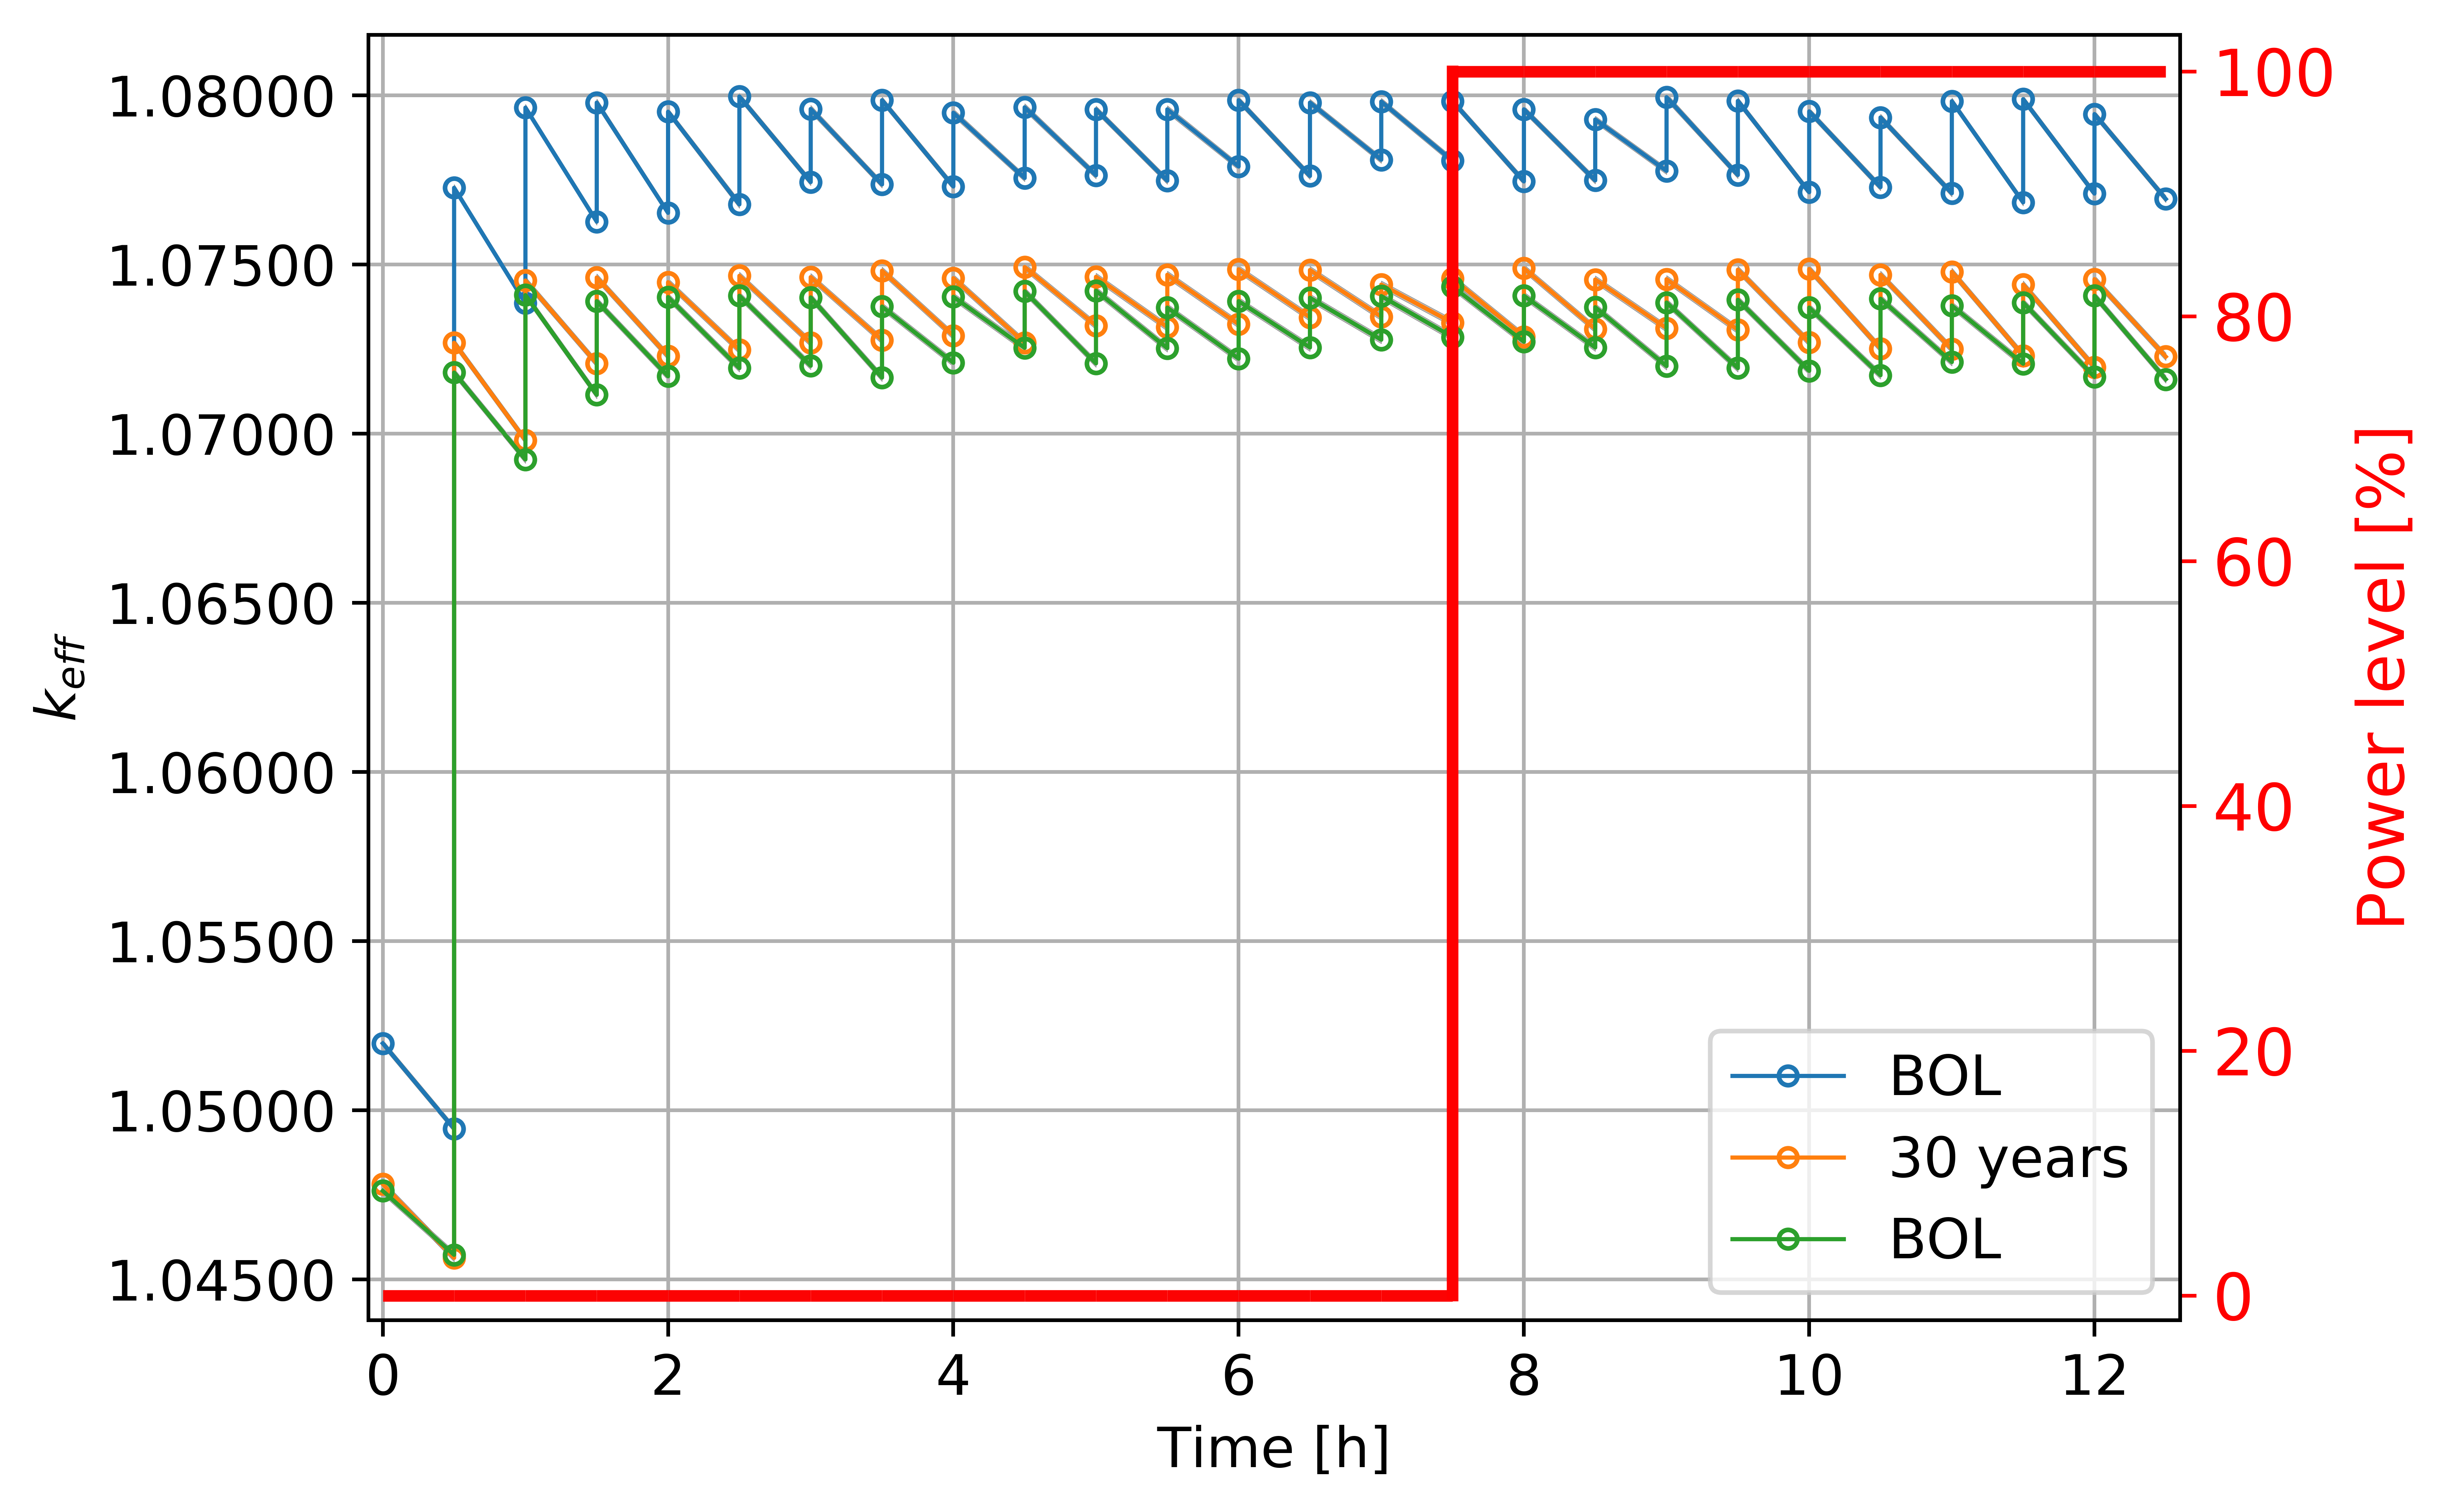
\includegraphics[width=0.905\textwidth]{ch6/kl100_keff.png}
\end{array}$
		\vspace{-5mm}
	\caption{SaltProc-calculated evolution of the effective multiplication 
	factor during the postulated load-following transient for various regimes 
	of the gas removal system operation. The uncertainty ($\pm\sigma=10$ $pcm$)
	is shaded.}
	\label{fig:msbr-lf-keff-evo}
\end{figure}

\begin{figure}[htbp!] % replace 't' with 'b' to 
	\centering
	$\begin{array}{r}
	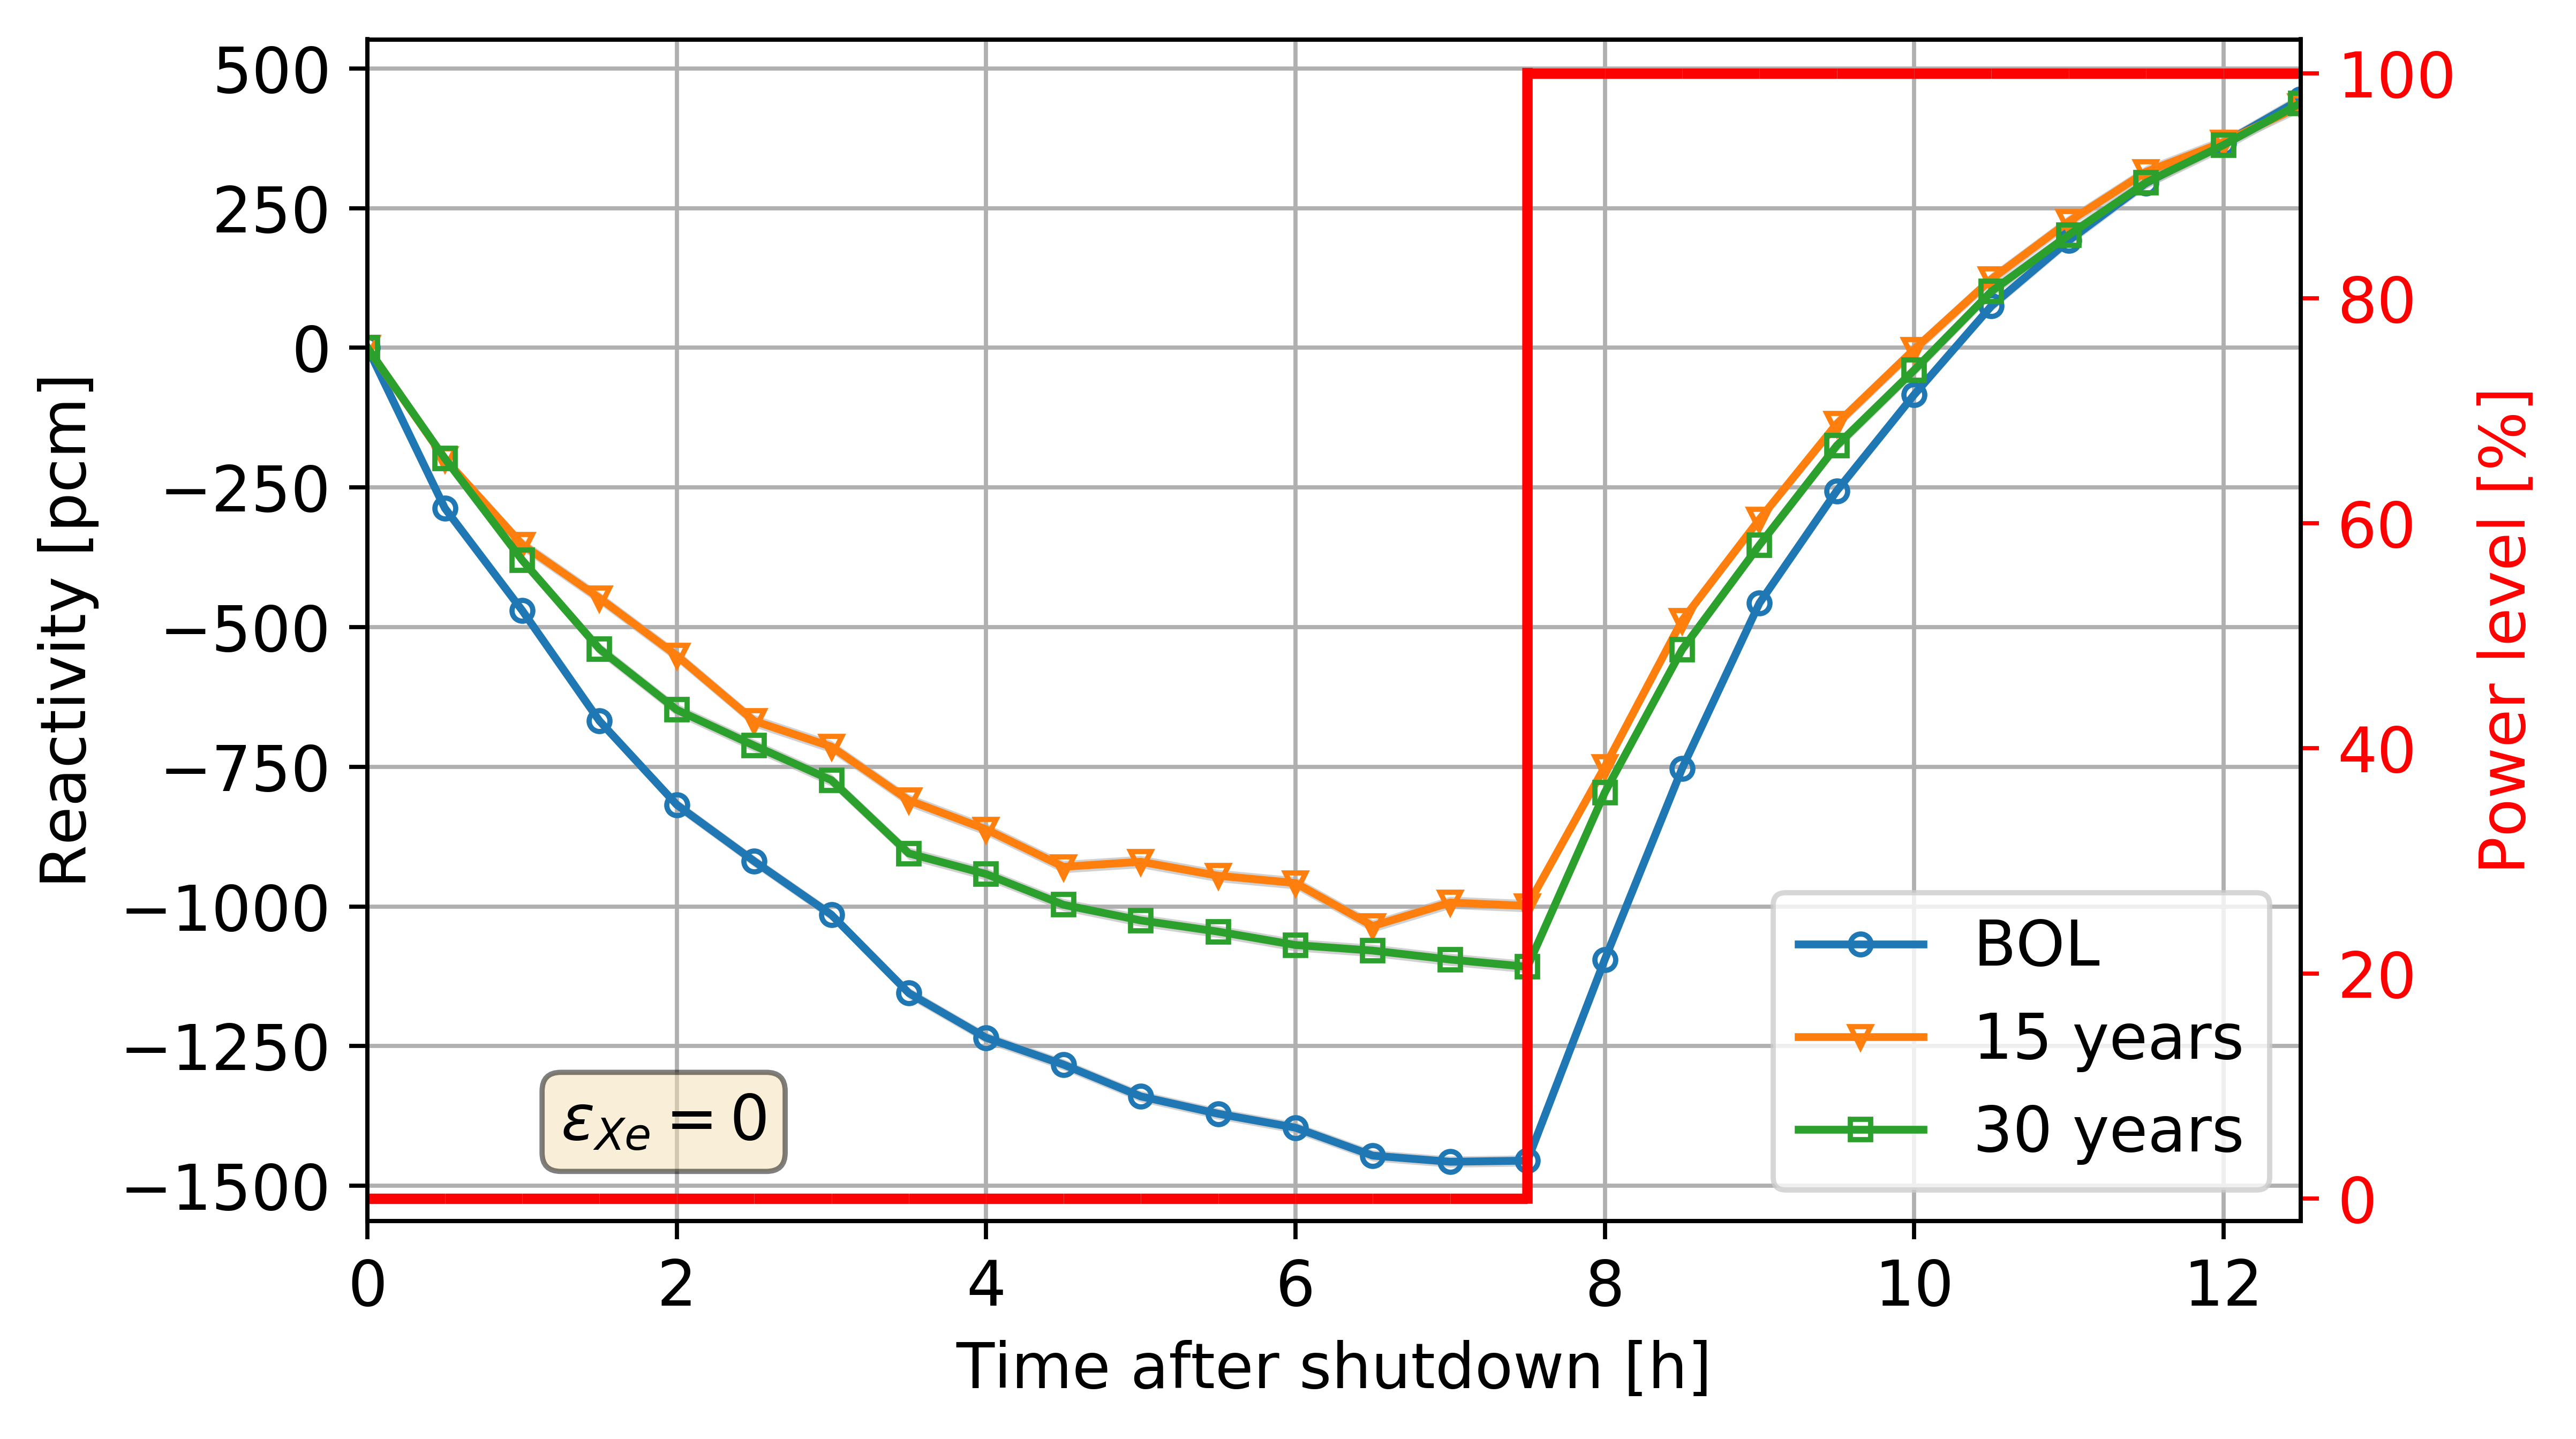
\includegraphics[width=0.923\textwidth]{ch6/kl1_rho.png}\vspace{-14mm}\\
	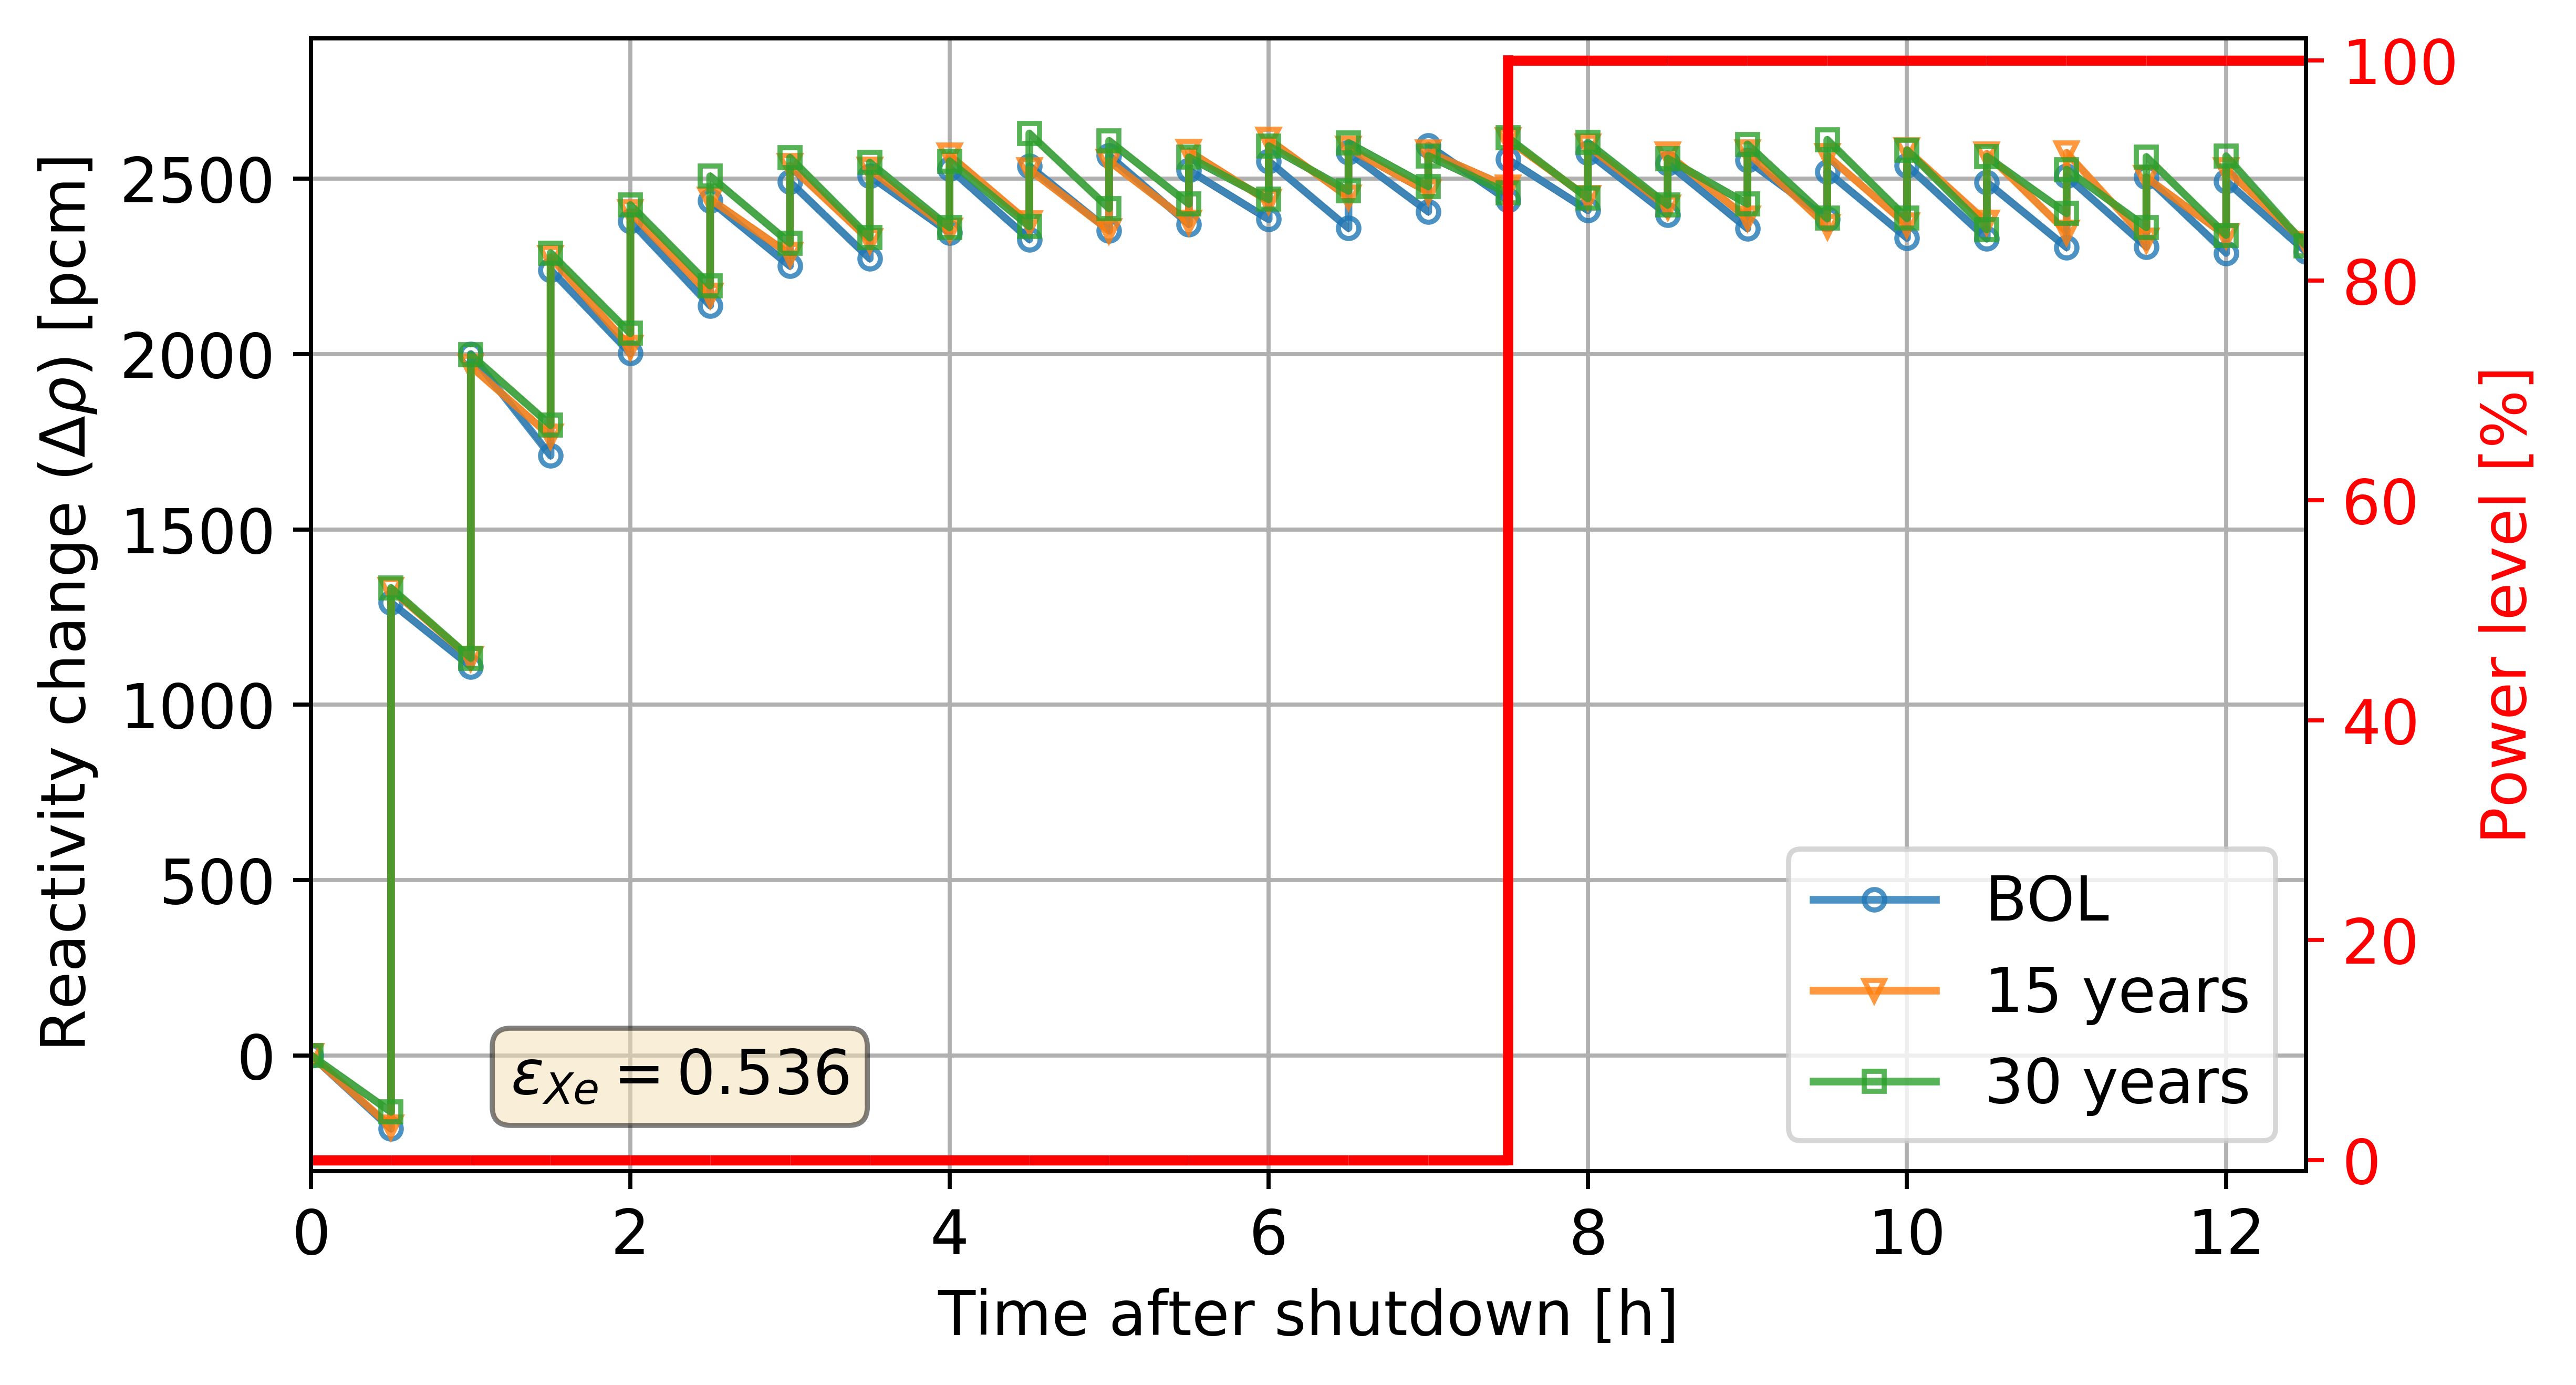
\includegraphics[width=0.9\textwidth]{ch6/kl25_rho.png}\vspace{-13mm}\\
	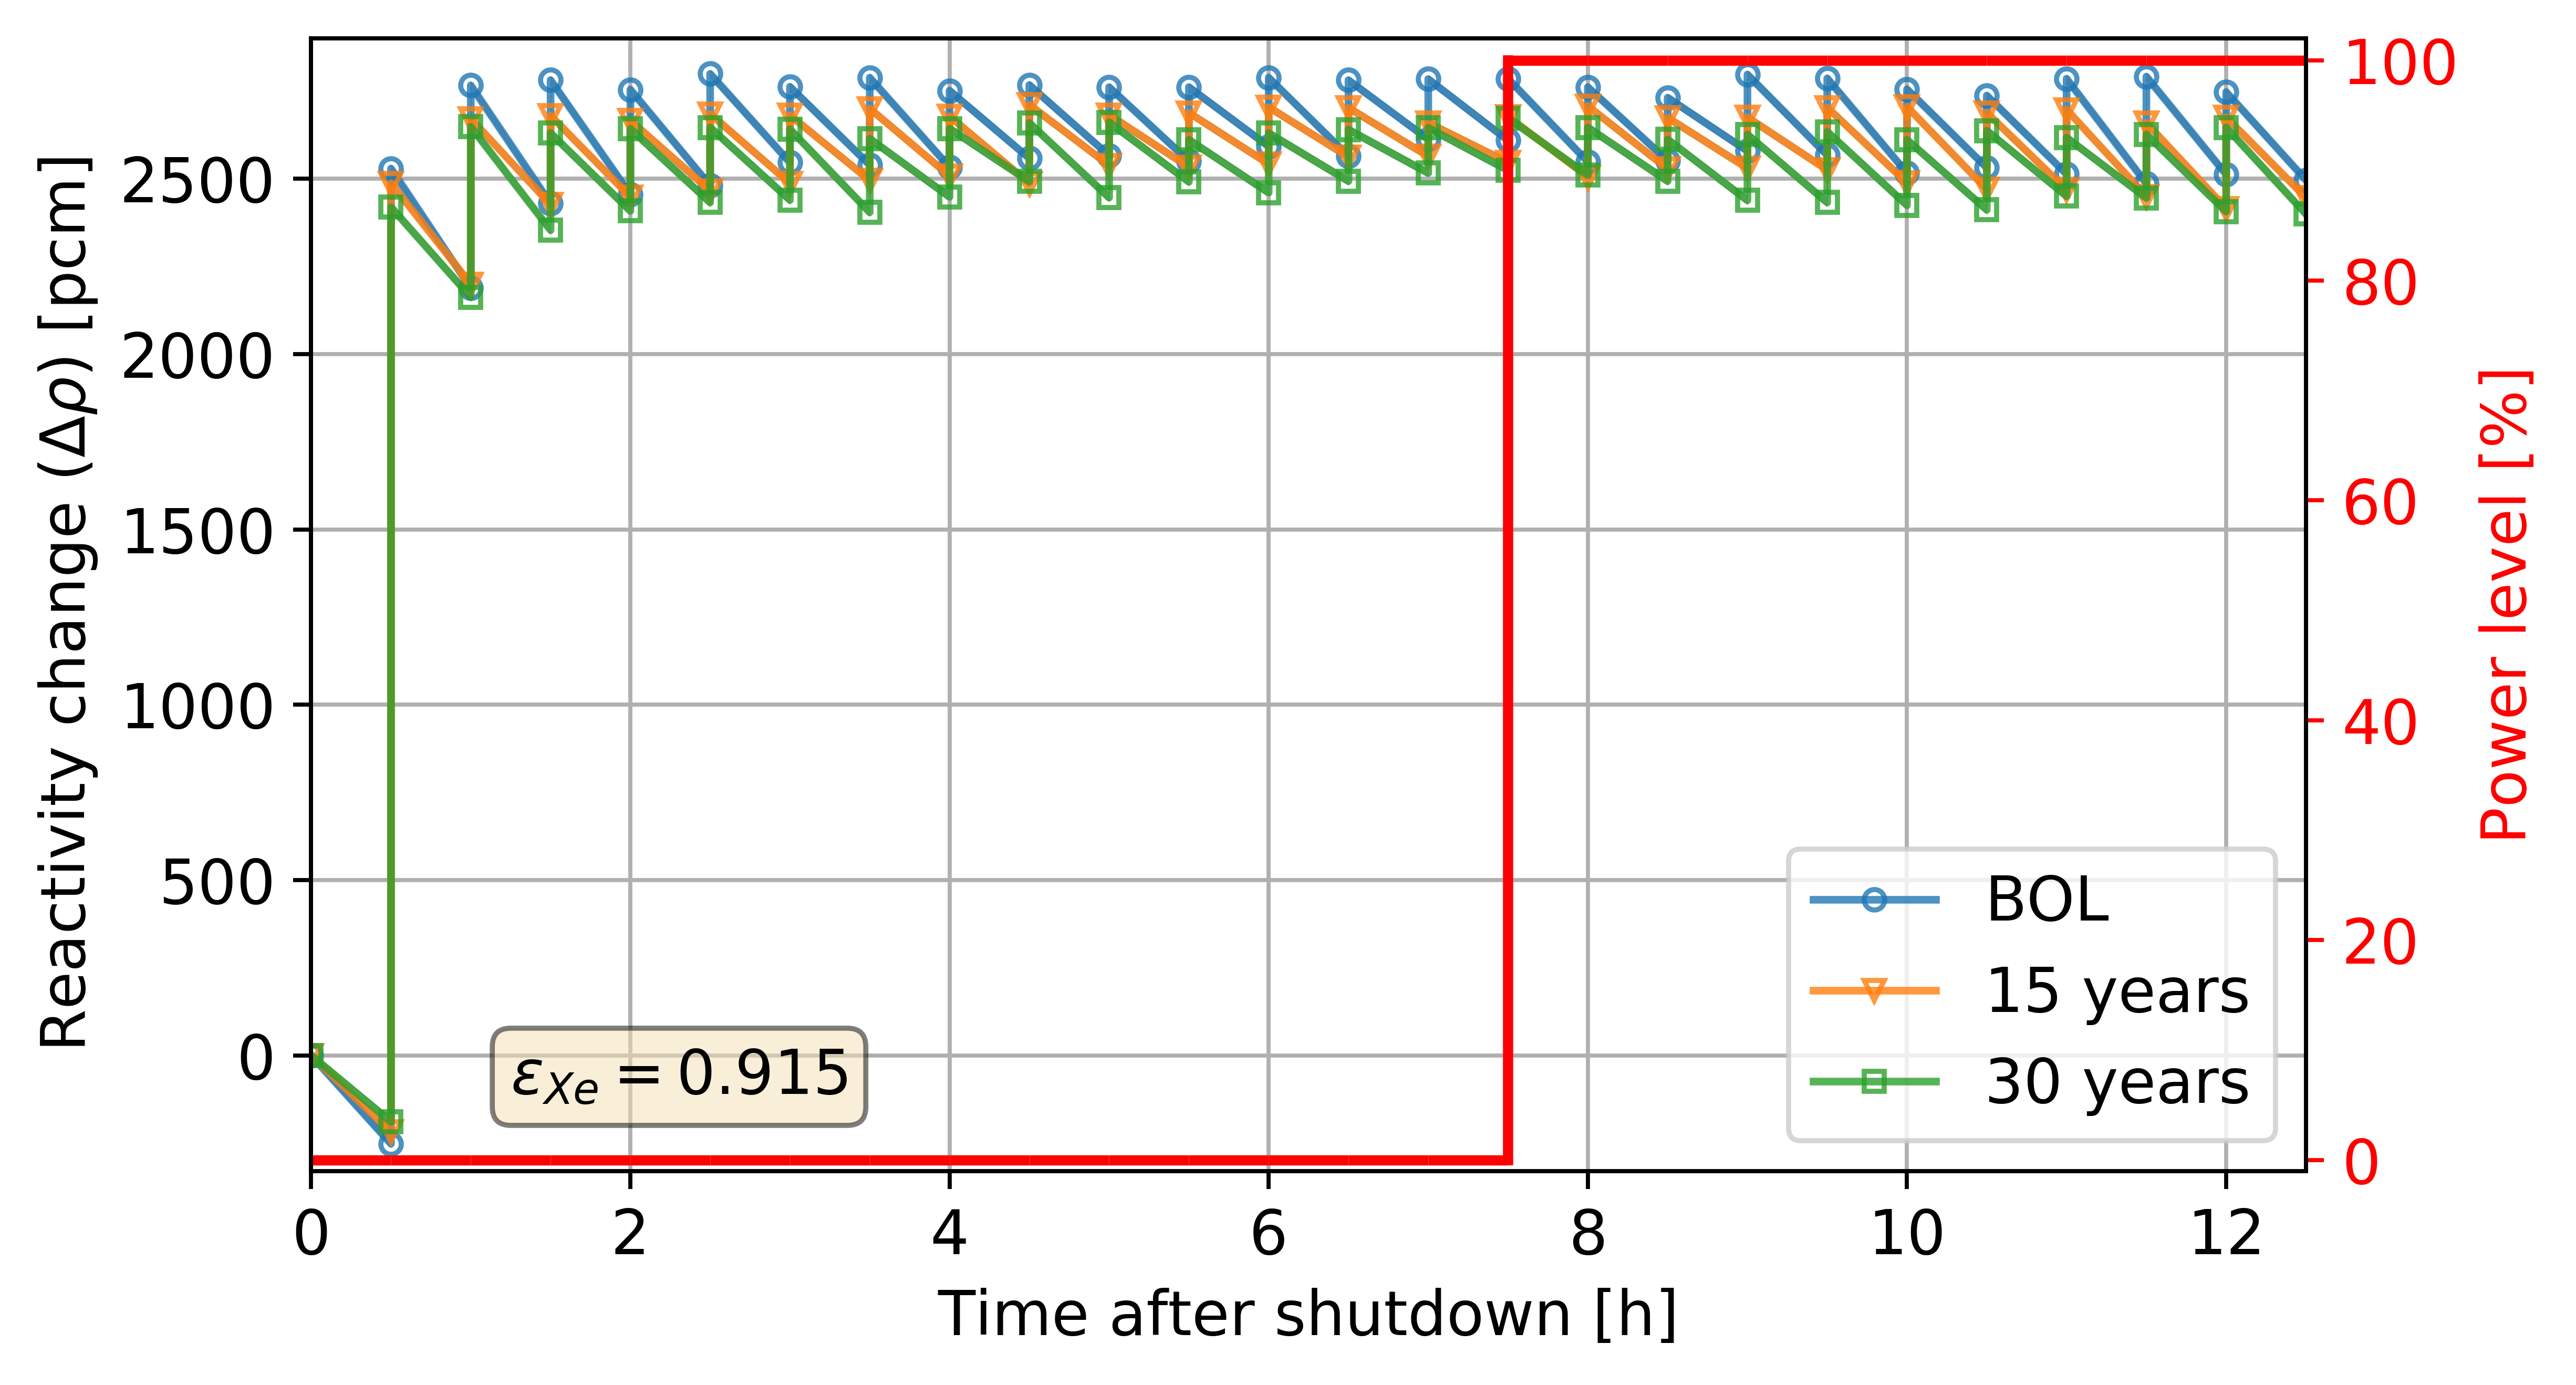
\includegraphics[width=0.9\textwidth]{ch6/kl100_rho.png}
	\end{array}$
	\vspace{-5mm}
	\caption{SaltProc-calculated evolution of the reactivity during the 
	postulated load-following transient for various regimes 
		of the gas removal system operation. The uncertainty ($\pm\sigma=10$ 
		$pcm$) is shaded.}
	\label{fig:msbr-lf-rho-evo}
\end{figure}
\FloatBarrier


\subsection{Fuel salt composition evolution}
Figure~\ref{fig:msbr-lf-xe-i-ratio} shows $^{135}$Xe and $^{135}$I mass 
dynamics evolution during the postulated transient for various gas removal 
efficiencies. The $^{135}$I/$^{135}$Xe concentration ratio at the beginning of 
the transient for the no-removal case is 2.45 and 2.03 at the \gls{BOL} and 
after 30 years of full-power operation, respectively. Because the
$^{135}$I/$^{135}$Xe concentration ratio is greater at startup, the $^{135}$Xe 
concentration peak is 11\% higher than at the \gls{EOL}, which is 
consistent with the \gls{TAP} \gls{MSR} results. However, a larger $^{135}$Xe 
concentration does not  necessarily worsen the xenon poisoning effect 
(Figure~\ref{fig:msbr-lf-rho-evo}) because the spectrum hardens toward 
\gls{EOL} and the $^{135}$Xe absorption cross section slumps with higher 
neutron energy (see Figure~\ref{fig:tap-pwr-spectrum}).

For the high gas removal efficiency regime, the $^{135}$I/$^{135}$Xe 
concentration ratio is 2.47 and 2.08 at the \gls{BOL} and after 
30 years of full-power operation, respectively. For the \gls{BOL} and a
30-year case, the $^{135}$Xe concentration peaked only by 8\% at the end of a 
first 30-minute depletion step, which caused a 189-$pcm$ negative reactivity 
insertion. Afterward, the concentration of $^{135}$Xe dropped quickly because 
the gas removal system extracted most of the fission gas. The $^{135}$Xe 
concentration in the fuel salt before the shutdown is approximately 7 times 
greater than after the power turned back on, which caused significant 
reactivity growth by $\approx2550$ $pcm$. Surprisingly, the removal of 12 g of 
$^{135}$Xe from $t=30min$ to $t=60min$ caused an impressive 2600-$pcm$ 
positive reactivity insertion (217 pcm/g$^{135}$Xe reactivity worth). 
\begin{figure}[htbp!] % replace 't' with 'b' to 
	\centering
	$\begin{array}{r}
	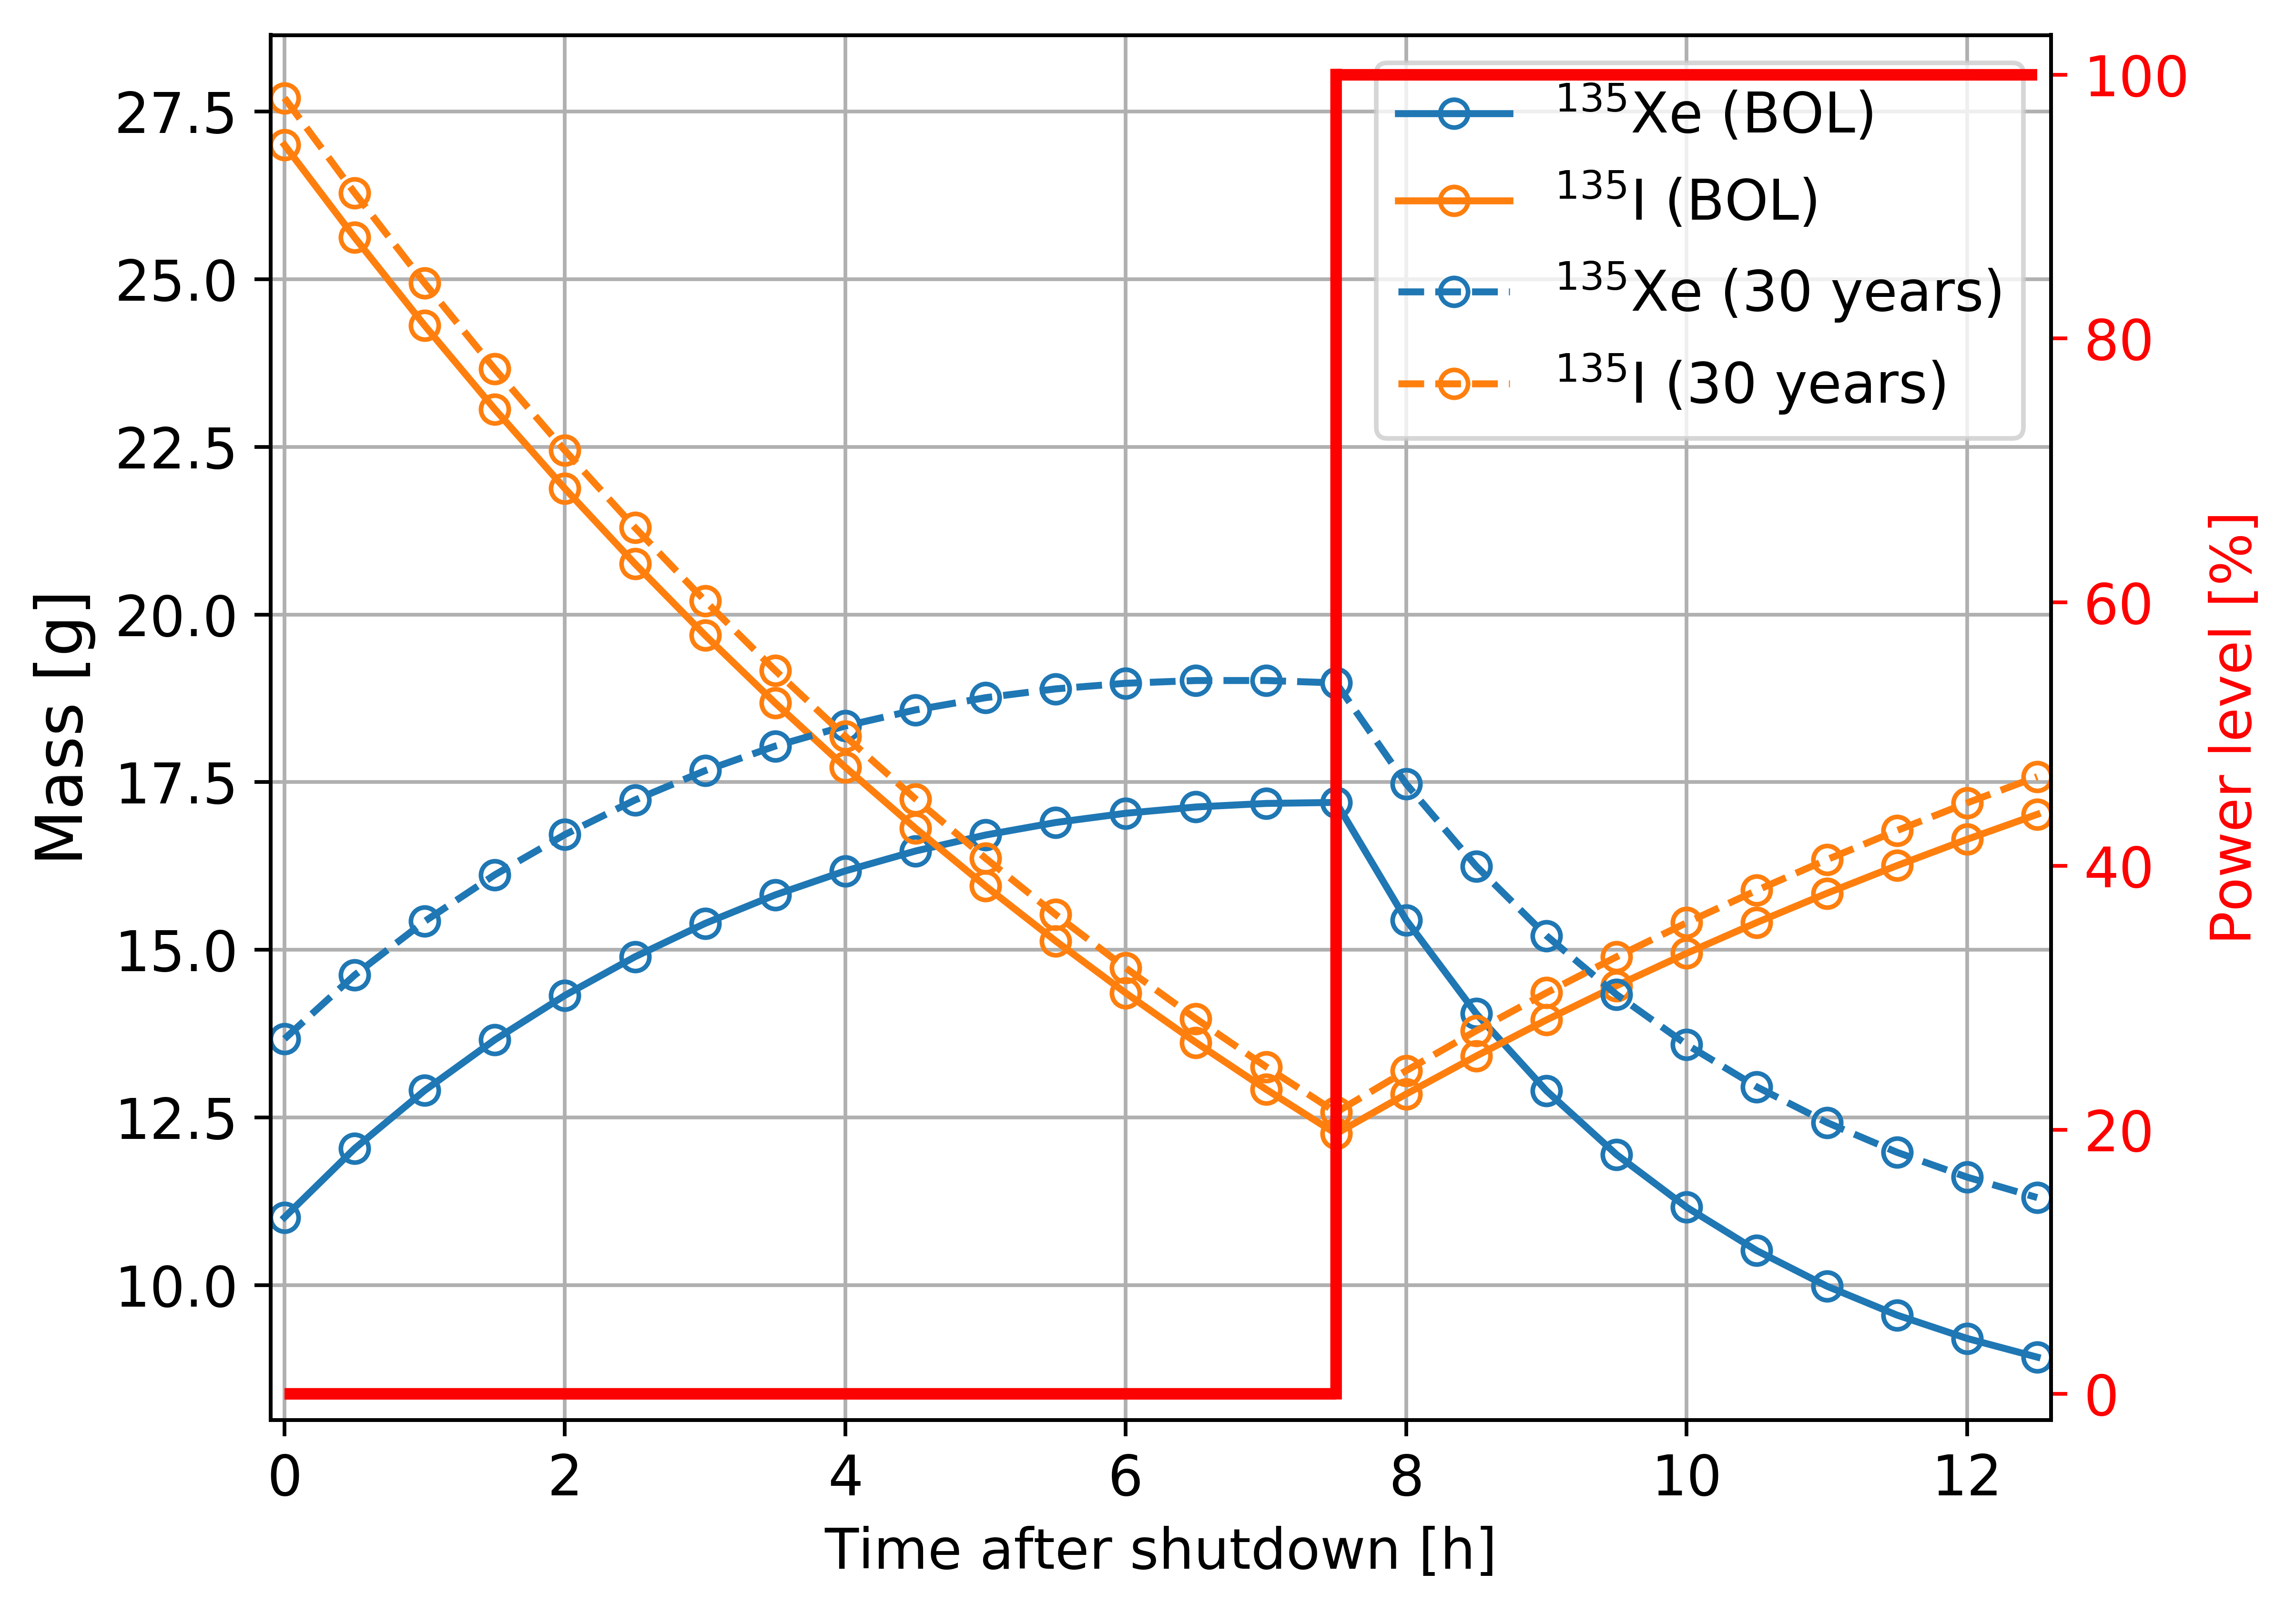
\includegraphics[width=0.86\textwidth]{ch6/kl1_xe_i_ratio.png}\vspace{-12mm}\\
	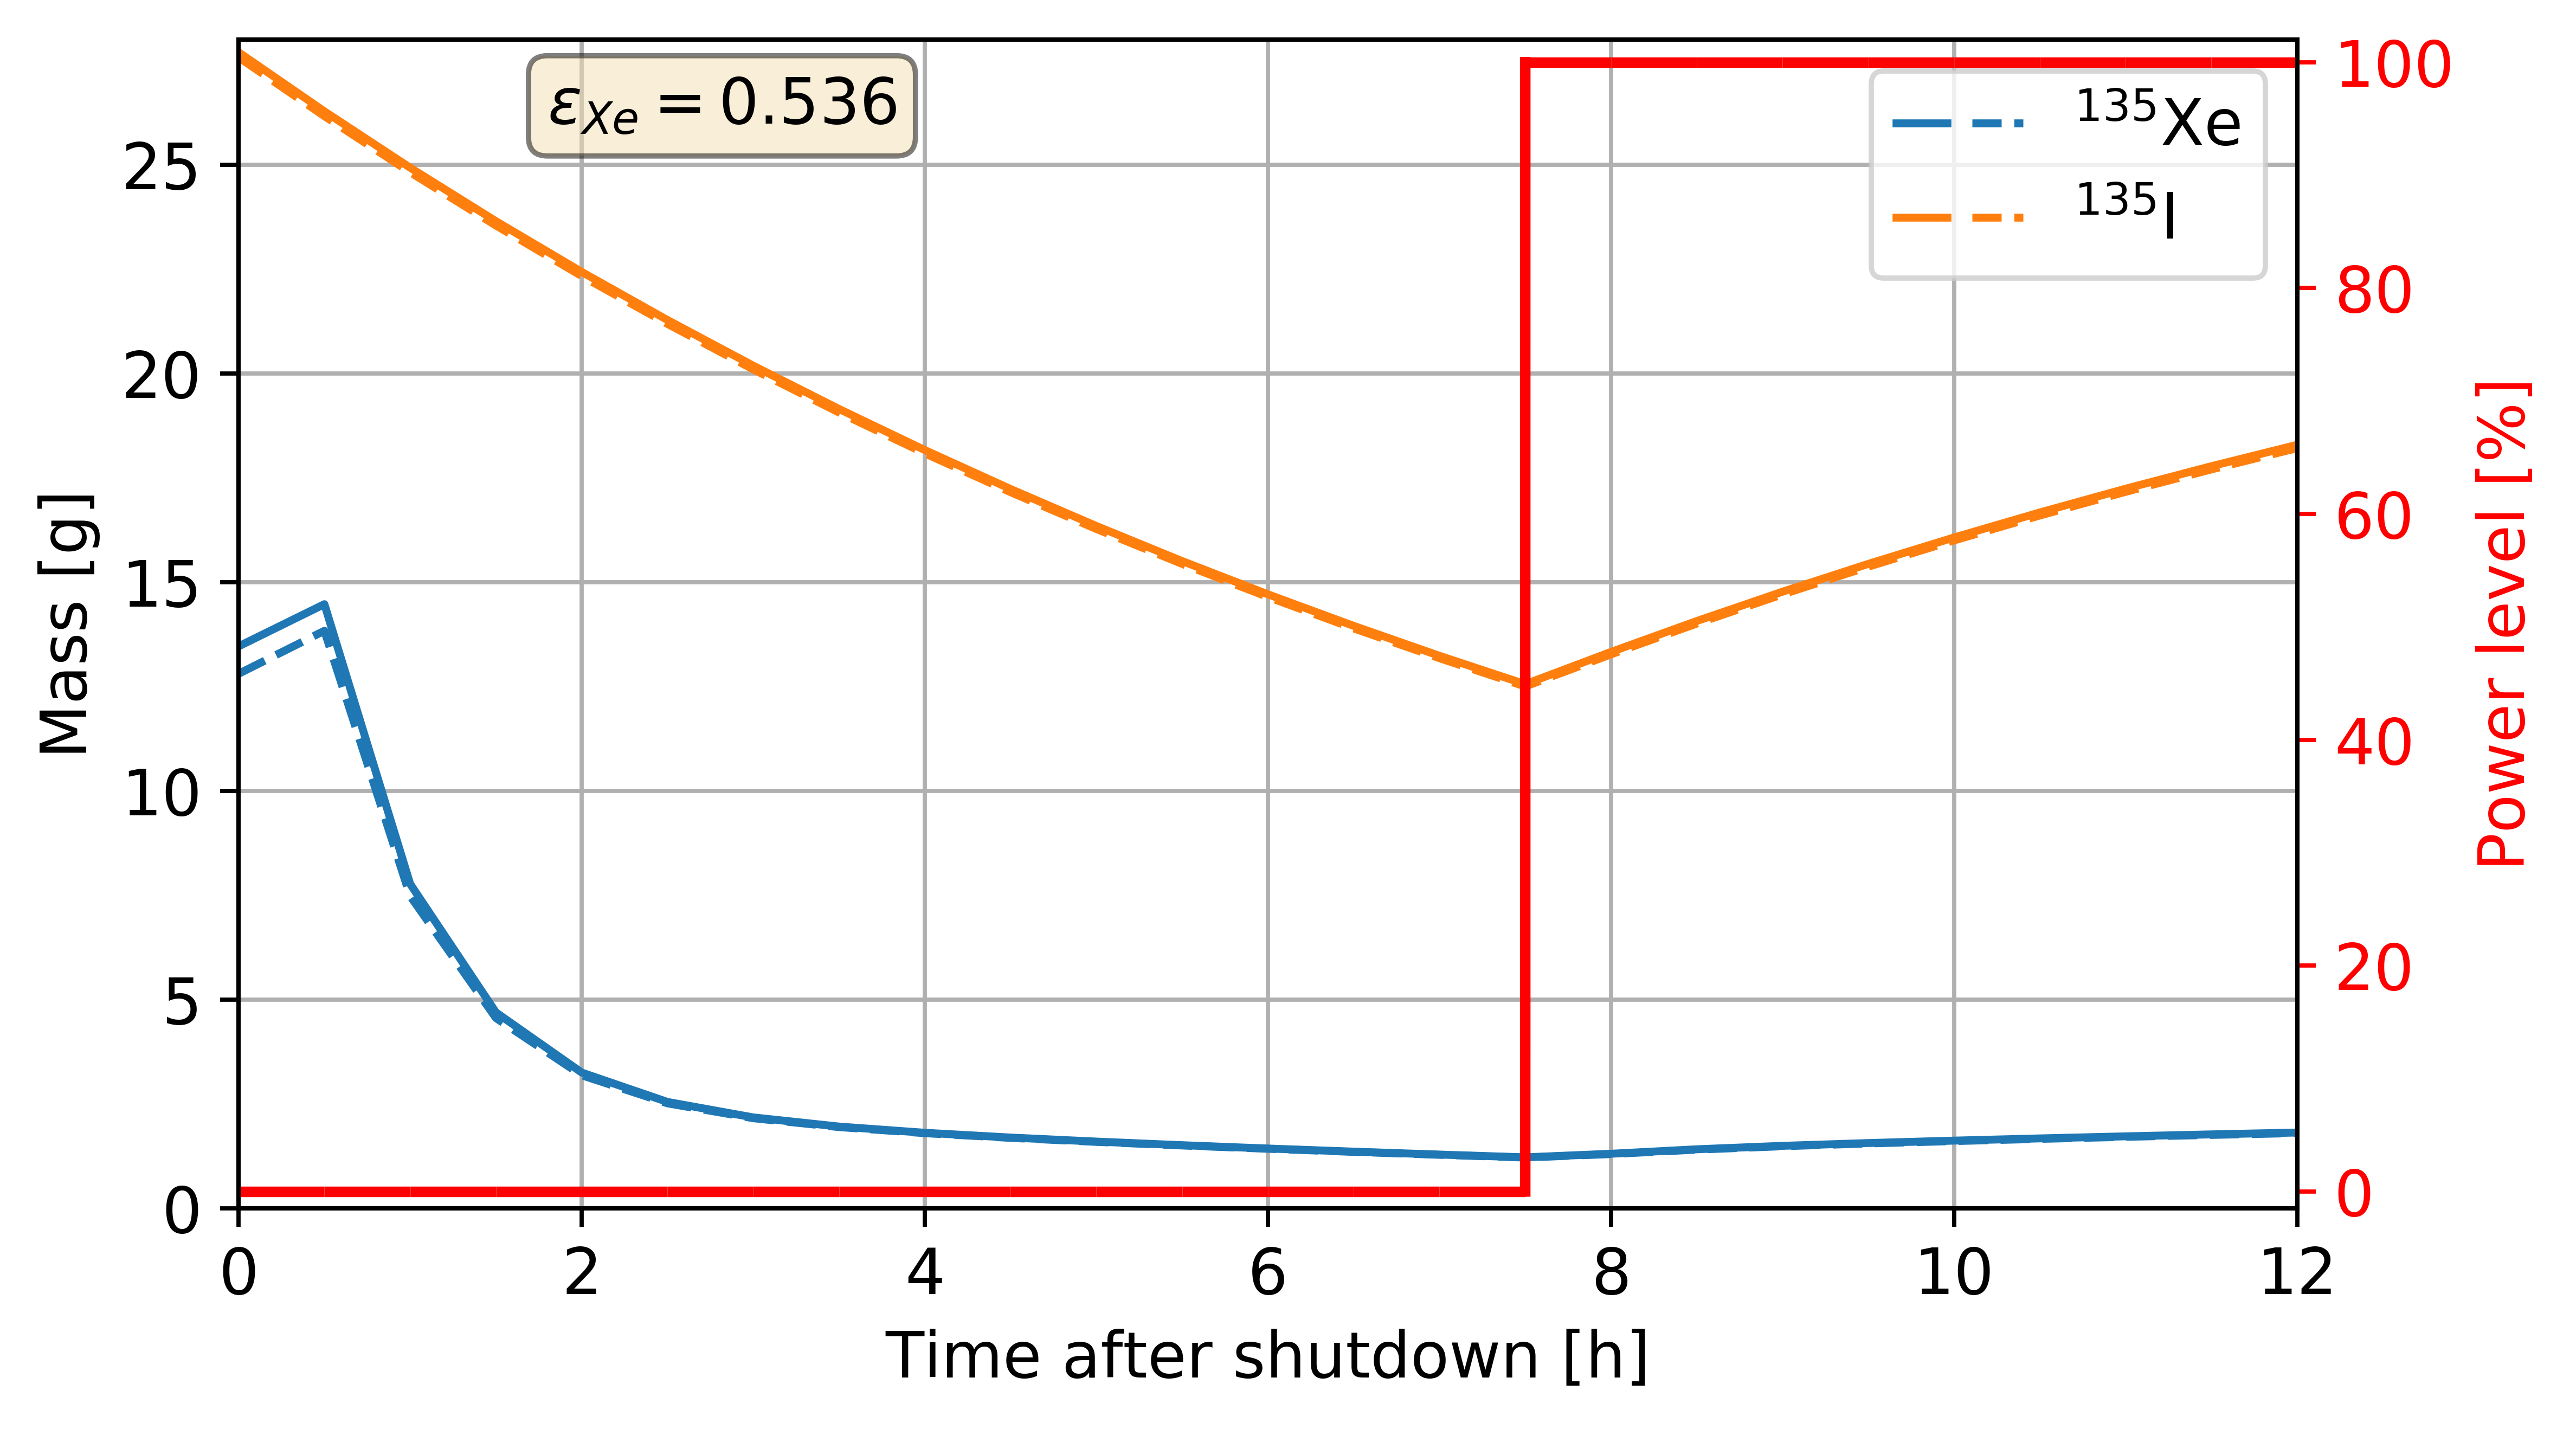
\includegraphics[width=0.86\textwidth]{ch6/kl25_xe_i_ratio.png}\vspace{-12mm}\\
	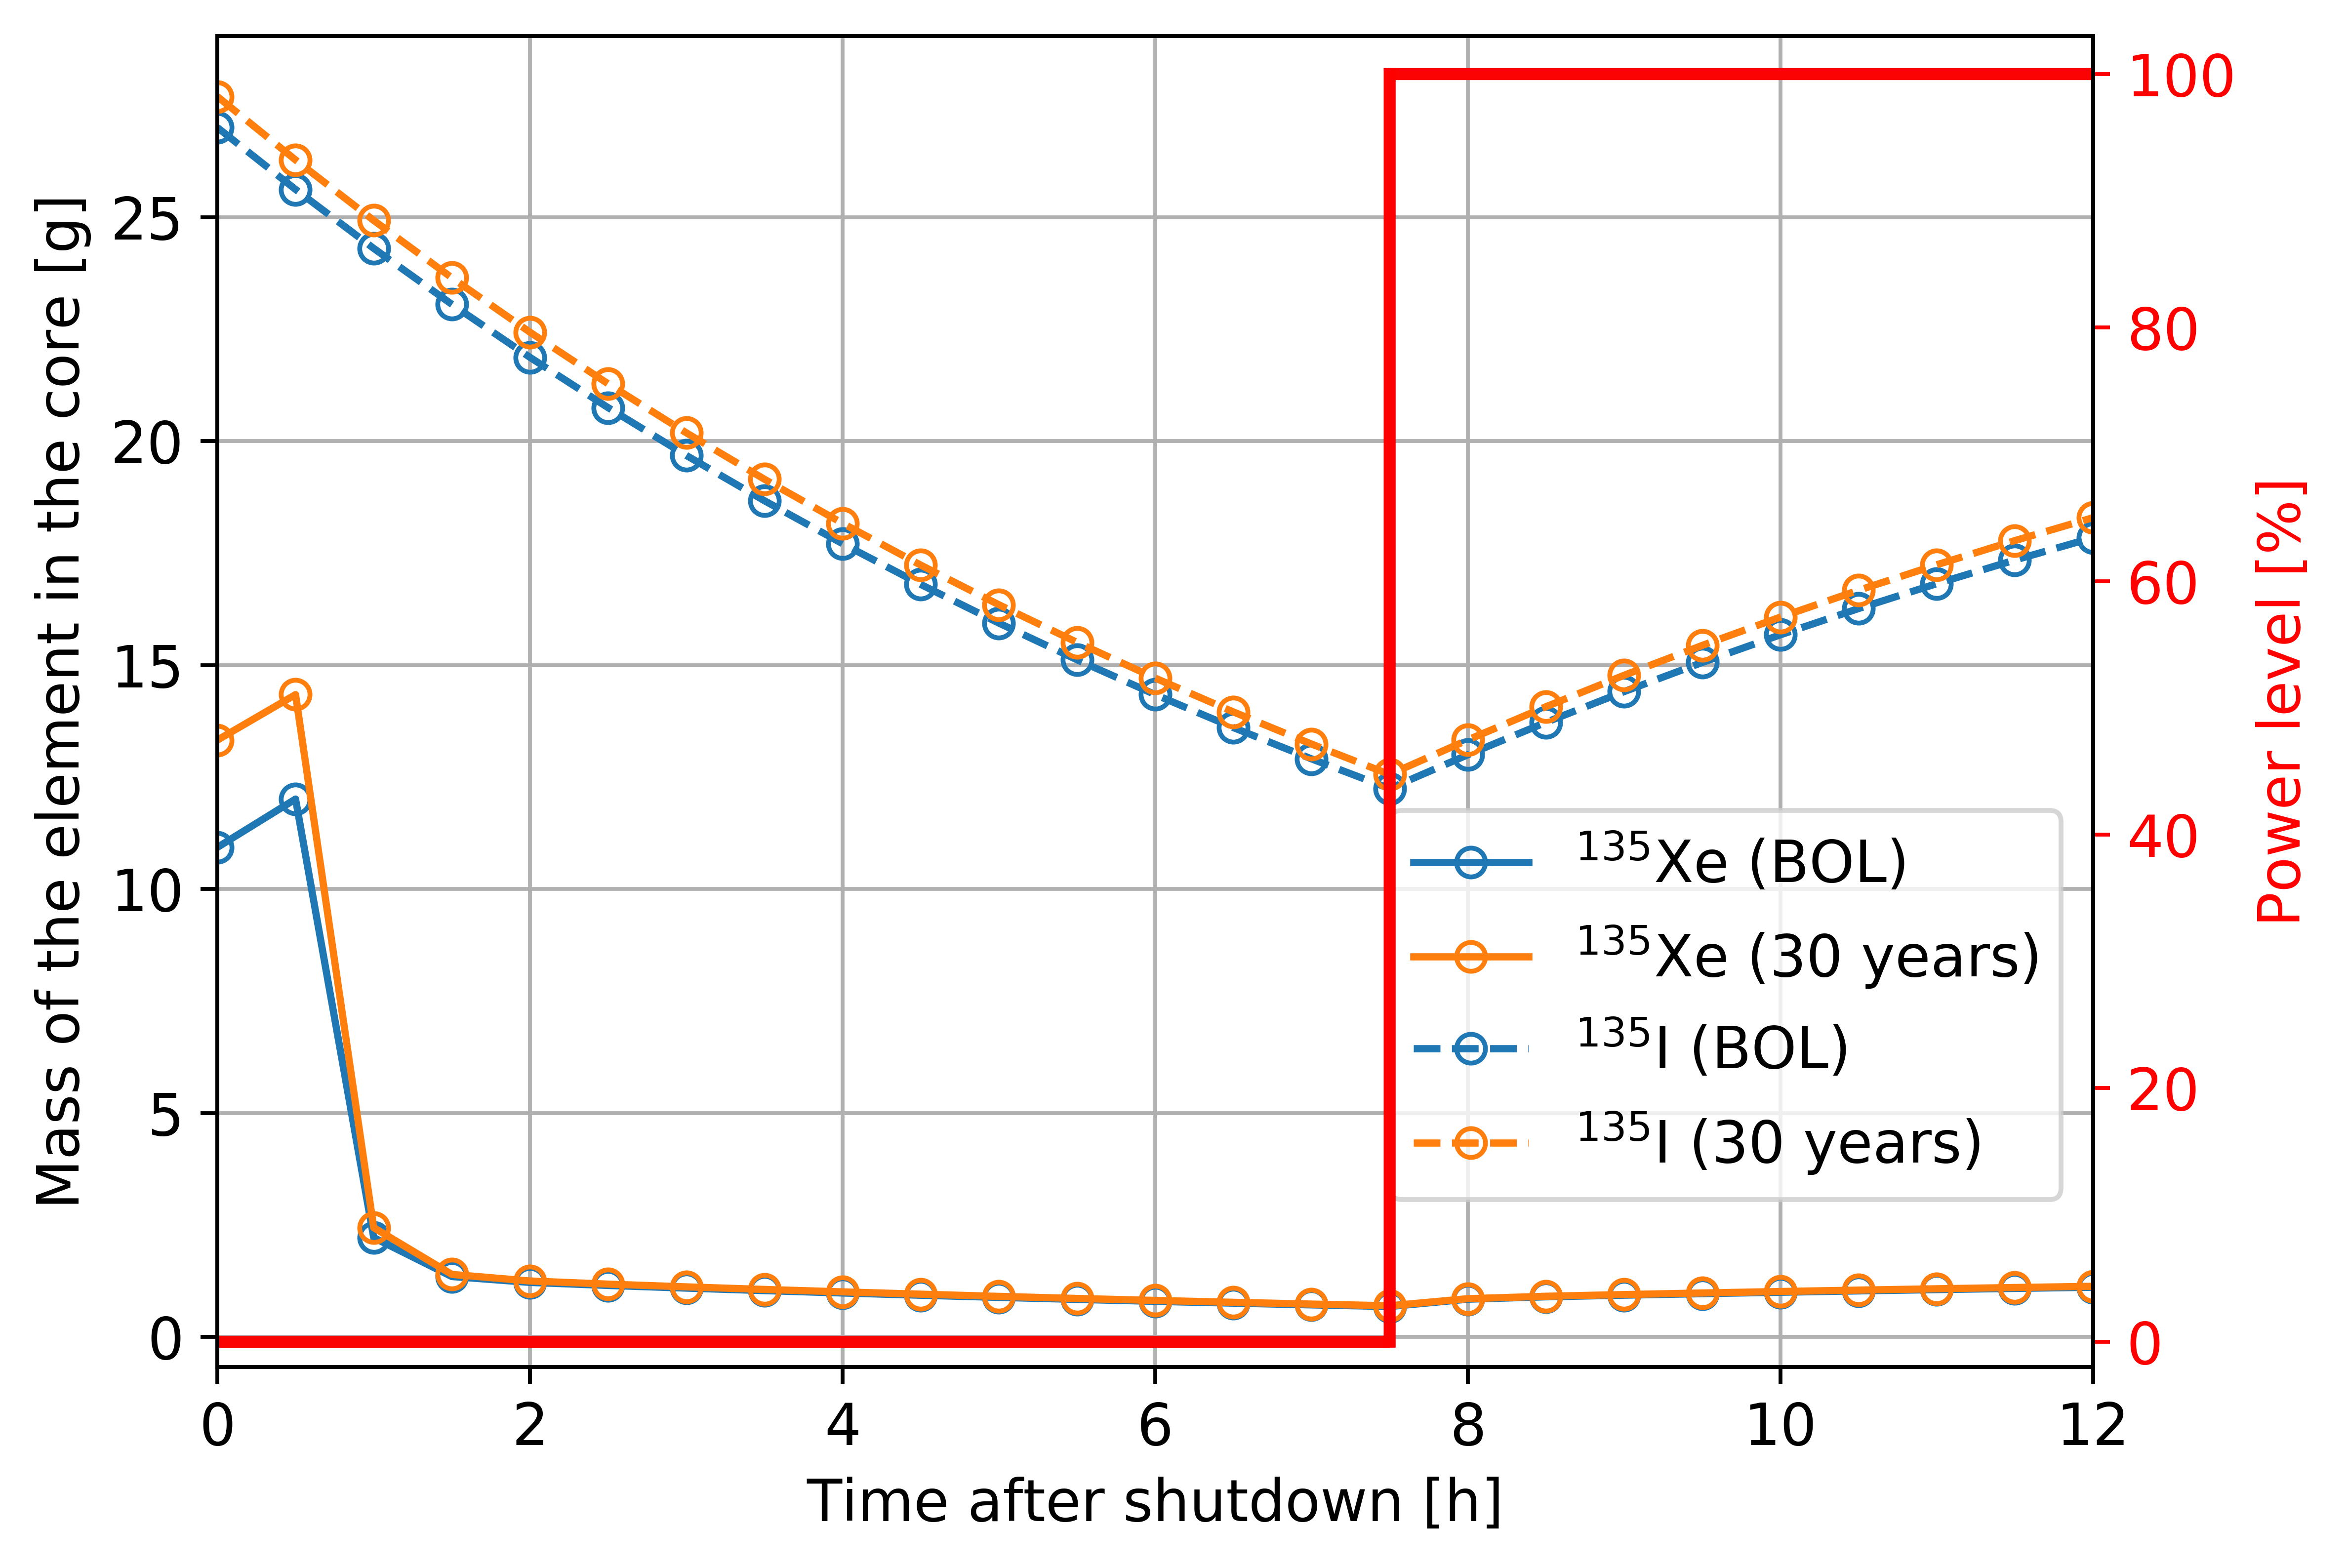
\includegraphics[width=0.86\textwidth]{ch6/kl100_xe_i_ratio.png}
	\end{array}$
	\vspace{-4mm}
	\caption{Comparison of $^{135}$Xe and $^{135}$I isotopic content at the 
		\gls{BOL} (dashed line) and after 30 years of operation (solid line) 
		for various gas removal regimes. Uncertainty of the predicted mass 
		will be estimated and discussed in Chapter 7.}
	\label{fig:msbr-lf-xe-i-ratio}
\end{figure}

Such large fluctuations in the $^{135}$Xe concentration are observed due 
to the batch-wise nature 
of SaltProc simulations (e.g., the fraction of target poison is being 
removed discretely at the end of each depletion step). Realistically, the gas 
removal system would extract gas from the fuel salt continuously, which would 
result in a much smoother change in the concentration and, accordingly, 
in the reactivity. Notably, for both \gls{BOL} and \gls{EOL}, the 
$^{135}$Xe mass stabilized at 1 g in about 3-4 hours after the shutdown and 
then inclined slowly ($60$ $mg/EFPH$) after power ramp-up from 0 to 100\%. 
That is, when the reactor returns to a full-power level,  the $^{135}$Xe 
concentration during a few days will be significantly lower than before the
load-following transient. Thus, fewer thermal neutrons will be parasitically 
absorbed in the fission gas. As a result, long-term fuel cycle performance 
metrics such as fuel utilization and core lifetime would benefit 
enormously from a very low $^{135}$Xe concentration in the core after the 
postulated transient. In other words, the transient cleans up the fuel salt, 
but more analyses are required to evaluate all benefits of this finding. 

In the case of moderate gas removal efficiency, the fission product 
concentration changes very similarly to a high removal efficiency case. The 
$^{135}$I/$^{135}$Xe concentration ratio is 2.15 and 2.06 at the \gls{BOL} and 
after 30 years of full-power operation, respectively, and caused a 7.5\% hike 
in $^{135}$Xe concentration. Surprisingly, a significantly lower gas removal 
efficiency ($\epsilon_{Xe}=0.536$ instead of 0.915) provided comparable 
benefits to the core neutronics during the postulated load-following 
transient. Similarly to the $\epsilon_{Xe}=0.915$ case, the 
$^{135}$Xe mass stabilized at 1.5 g about 5 hours after the shutdown and 
then increased slowly ($165$ $mg/EFPH$) after power ramp-up from 0 to 100\%.
In conclusion, a simpler and cheaper gas removal system with extraction 
efficiency $\epsilon_{Xe}=0.536$ is sufficient to suppress the xenon 
poisoning effect to an acceptable level (-161 $pcm$) and improve the 
load-following capability of the \gls{MSBR}.


\subsection{Neutron spectrum}
Figure~\ref{fig:ch6-msbr-spectrum} shows that the \gls{MSBR} spectrum after 30 
years of operation (solid line) is harder than at the startup (dashed line). 
Compared with the \gls{MSBR}, the \gls{TAP} \gls{MSR} spectrum is 
significantly harder even when all moderator rods are inserted to the core. 
Notably, the \gls{MSBR} spectrum has a clear peak in the thermal energy 
region, but flat neutron energy dependence in intermediate and fast energy 
region, which is quite common for thermal reactors. In contrast, the \gls{TAP} 
core spectrum at the \gls{EOL} has a high peak in the fast and lower peak in 
the thermal energy region, which is typical for epithermal/intermediate 
reactors. This is the main reason why for the postulated load-following 
transient, I observed a significant xenon poisoning effect in the \gls{MSBR} 
and negligible xenon impact in the \gls{TAP} \gls{MSR} (see Chapter 5).
\begin{figure}[htbp!] % replace 't' with 'b' to 
	\centering
	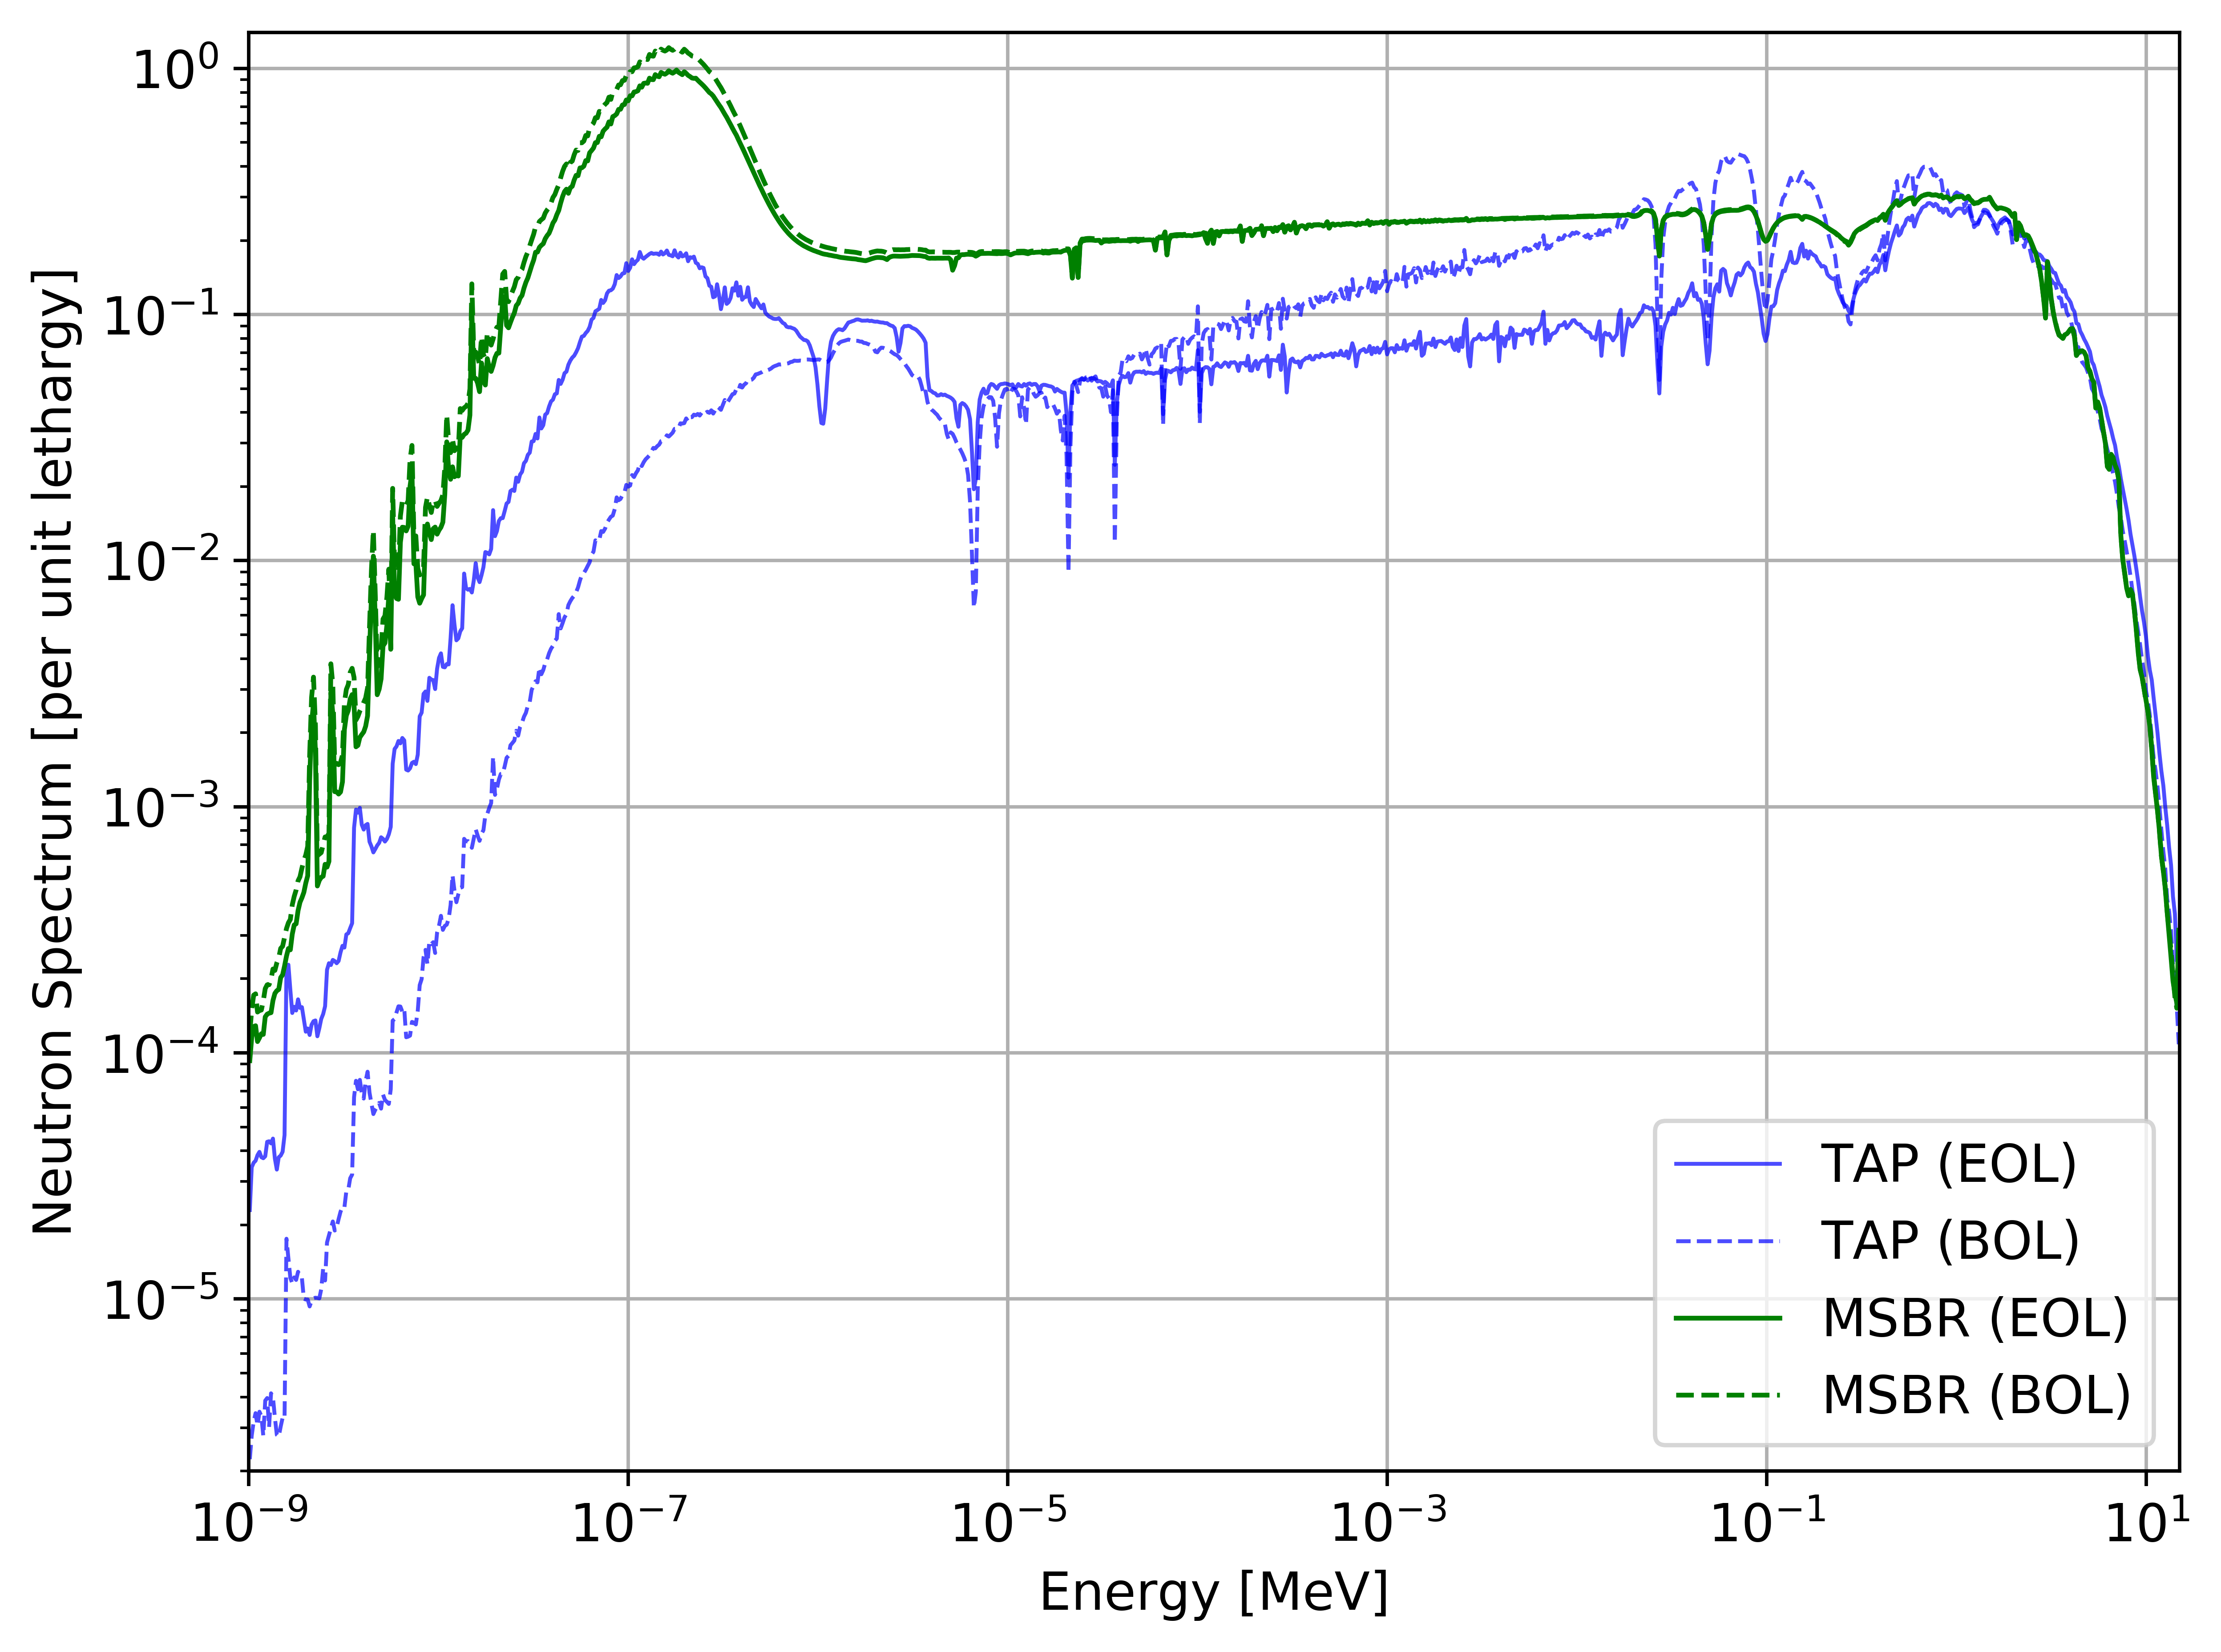
\includegraphics[width=\textwidth]{ch6/msbr_vs_tap_spectrum.png}
	\caption{Neutron spectra normalized by lethargy for the \gls{MSBR} and 
		\gls{TAP} at various moments during operation. The neutron flux 
		uncertainties $\sigma_{\Phi}$ are 0.6\% and 0.18\% for the \gls{TAP} 
		reactor and \gls{MSBR}, respectively.}
	\label{fig:ch6-msbr-spectrum}
\end{figure}

Any graphite-moderated liquid-fueled \gls{MSR} conceptual 
design\footnote{Integral Molten Salt Reactor (IMSR) from Terrestial Energy 
\cite{leblanc_integral_nodate}, Molten Salt Demonstration Reactor (MSDR) from 
Oak Ridge National Laboratory \cite{bettis_design_1972}, Liquid fluoride 
thorium reactor (LFTR) from Flibe energy \cite{sorensen_liquid-fluoride_2016}, 
etc.} would potentially demonstrate similar benefits from an online noble gas 
removal from the fuel salt.


\section{Safety and operational parameters}
The significant change of strong absorber concentrations in the fuel slightly 
shifts the core spectrum, potentially impacting the reactor's safety.
Since rapid changes in the fuel salt composition cannot be allowed to 
compromise critical safety margins,
I calculated major safety and operational parameters at various moments 
throughout the postulated transient using approaches from 
Sections~\ref{sec:safety-param} and \ref{ch5:saf_param}. 
The total temperature coefficient of reactivity ($\alpha_{ISO}$) must remain 
negative, and the total control rod worth (CRW) must be sufficient to trip the 
reactor throughout the postulated transient. Ideally, we want major safety 
and operational parameters to stay almost constant because the changes in 
those parameters would require fast response from the reactor control systems 
(i.e., control rod jerk in response to a CRW change).

\subsection{Temperature coefficient of reactivity}
Figure~\ref{fig:msbr-lf-tc-evo} shows the temperature feedback coefficient 
dynamics for the \gls{MSBR} during the transient for various gas removal 
efficiencies ($\epsilon_{Xe}=0.536$ and 0.915). 
The Fuel Temperature Coefficient ($\alpha_{T,F}$) becomes less strong at the 
beginning of the transient for all cases. The reason for this is a 
slight spectrum hardening due to the $^{135}$Xe concentration peak that 
changed the Doppler broadening of resonances. After that, the magnitude of 
$\alpha_{T,F}$ slowly increased due to a steady incline in the $^{135}$Xe 
concentration.
\begin{figure}[htbp!] % replace 't' with 'b' to 
	\centering
	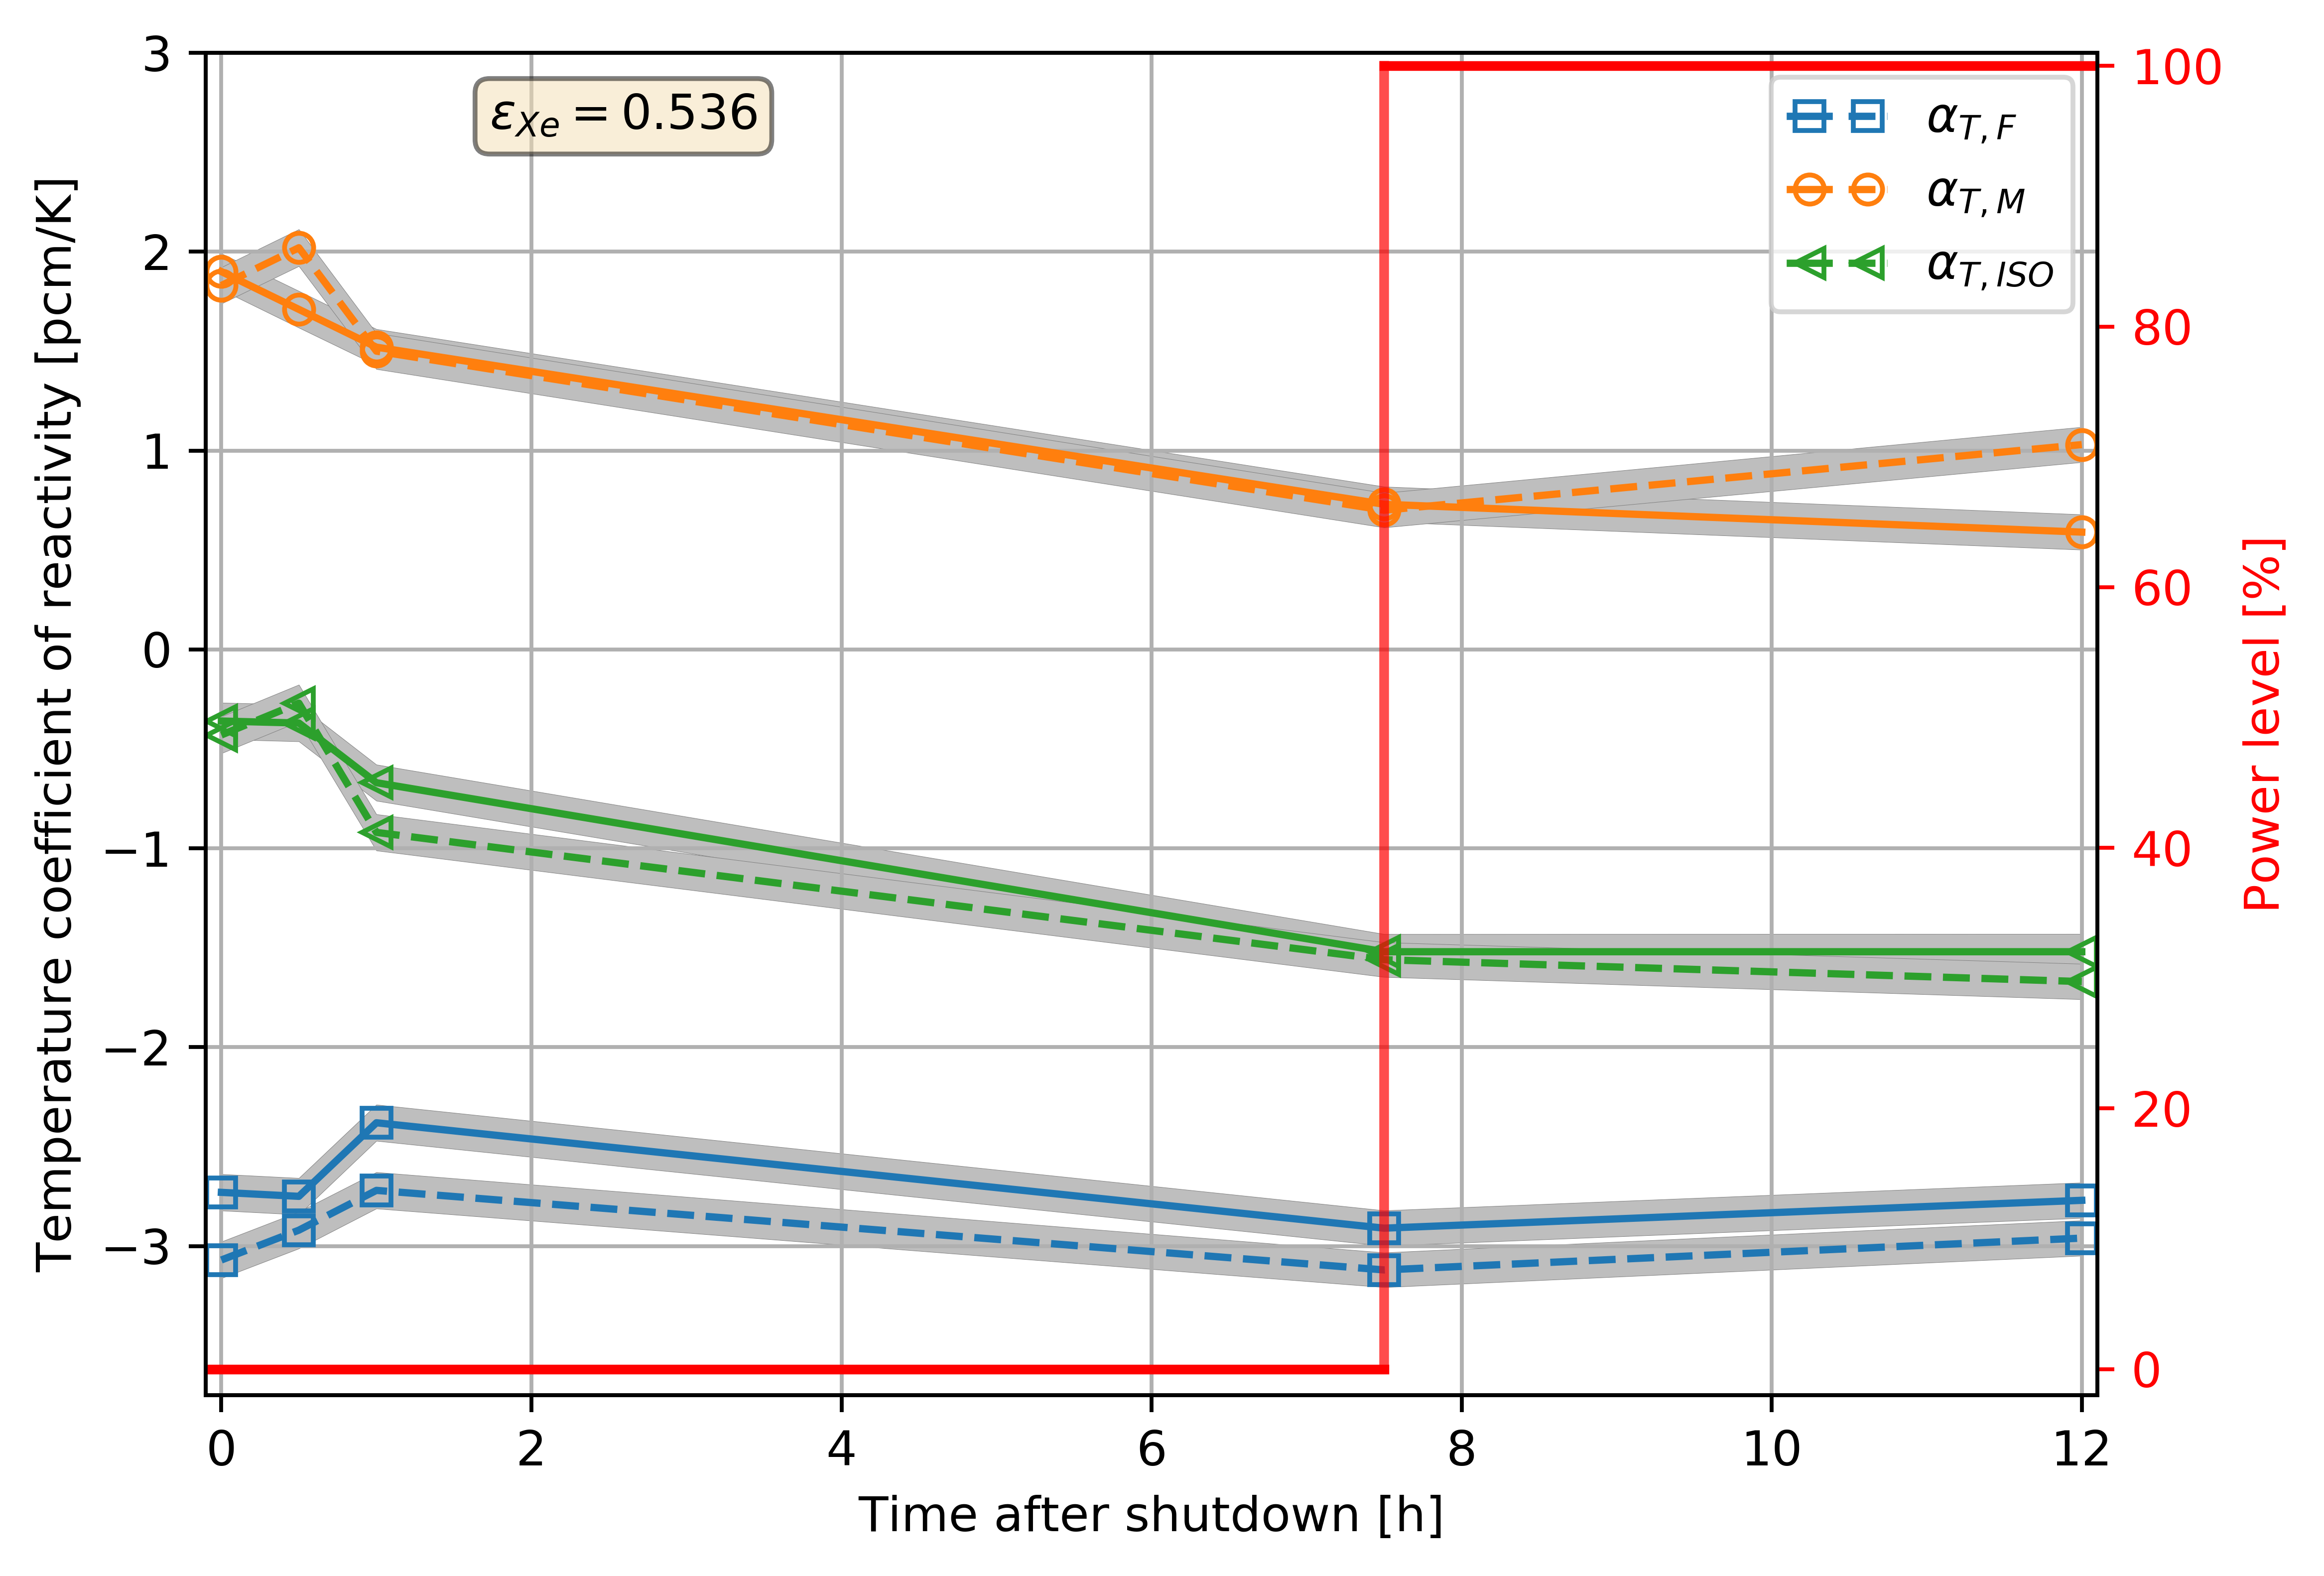
\includegraphics[width=0.95\textwidth]{ch6/saf_par/tc_evo_kl25.png}\\
	\vspace{-12mm}
	\hspace{+0.05mm}
	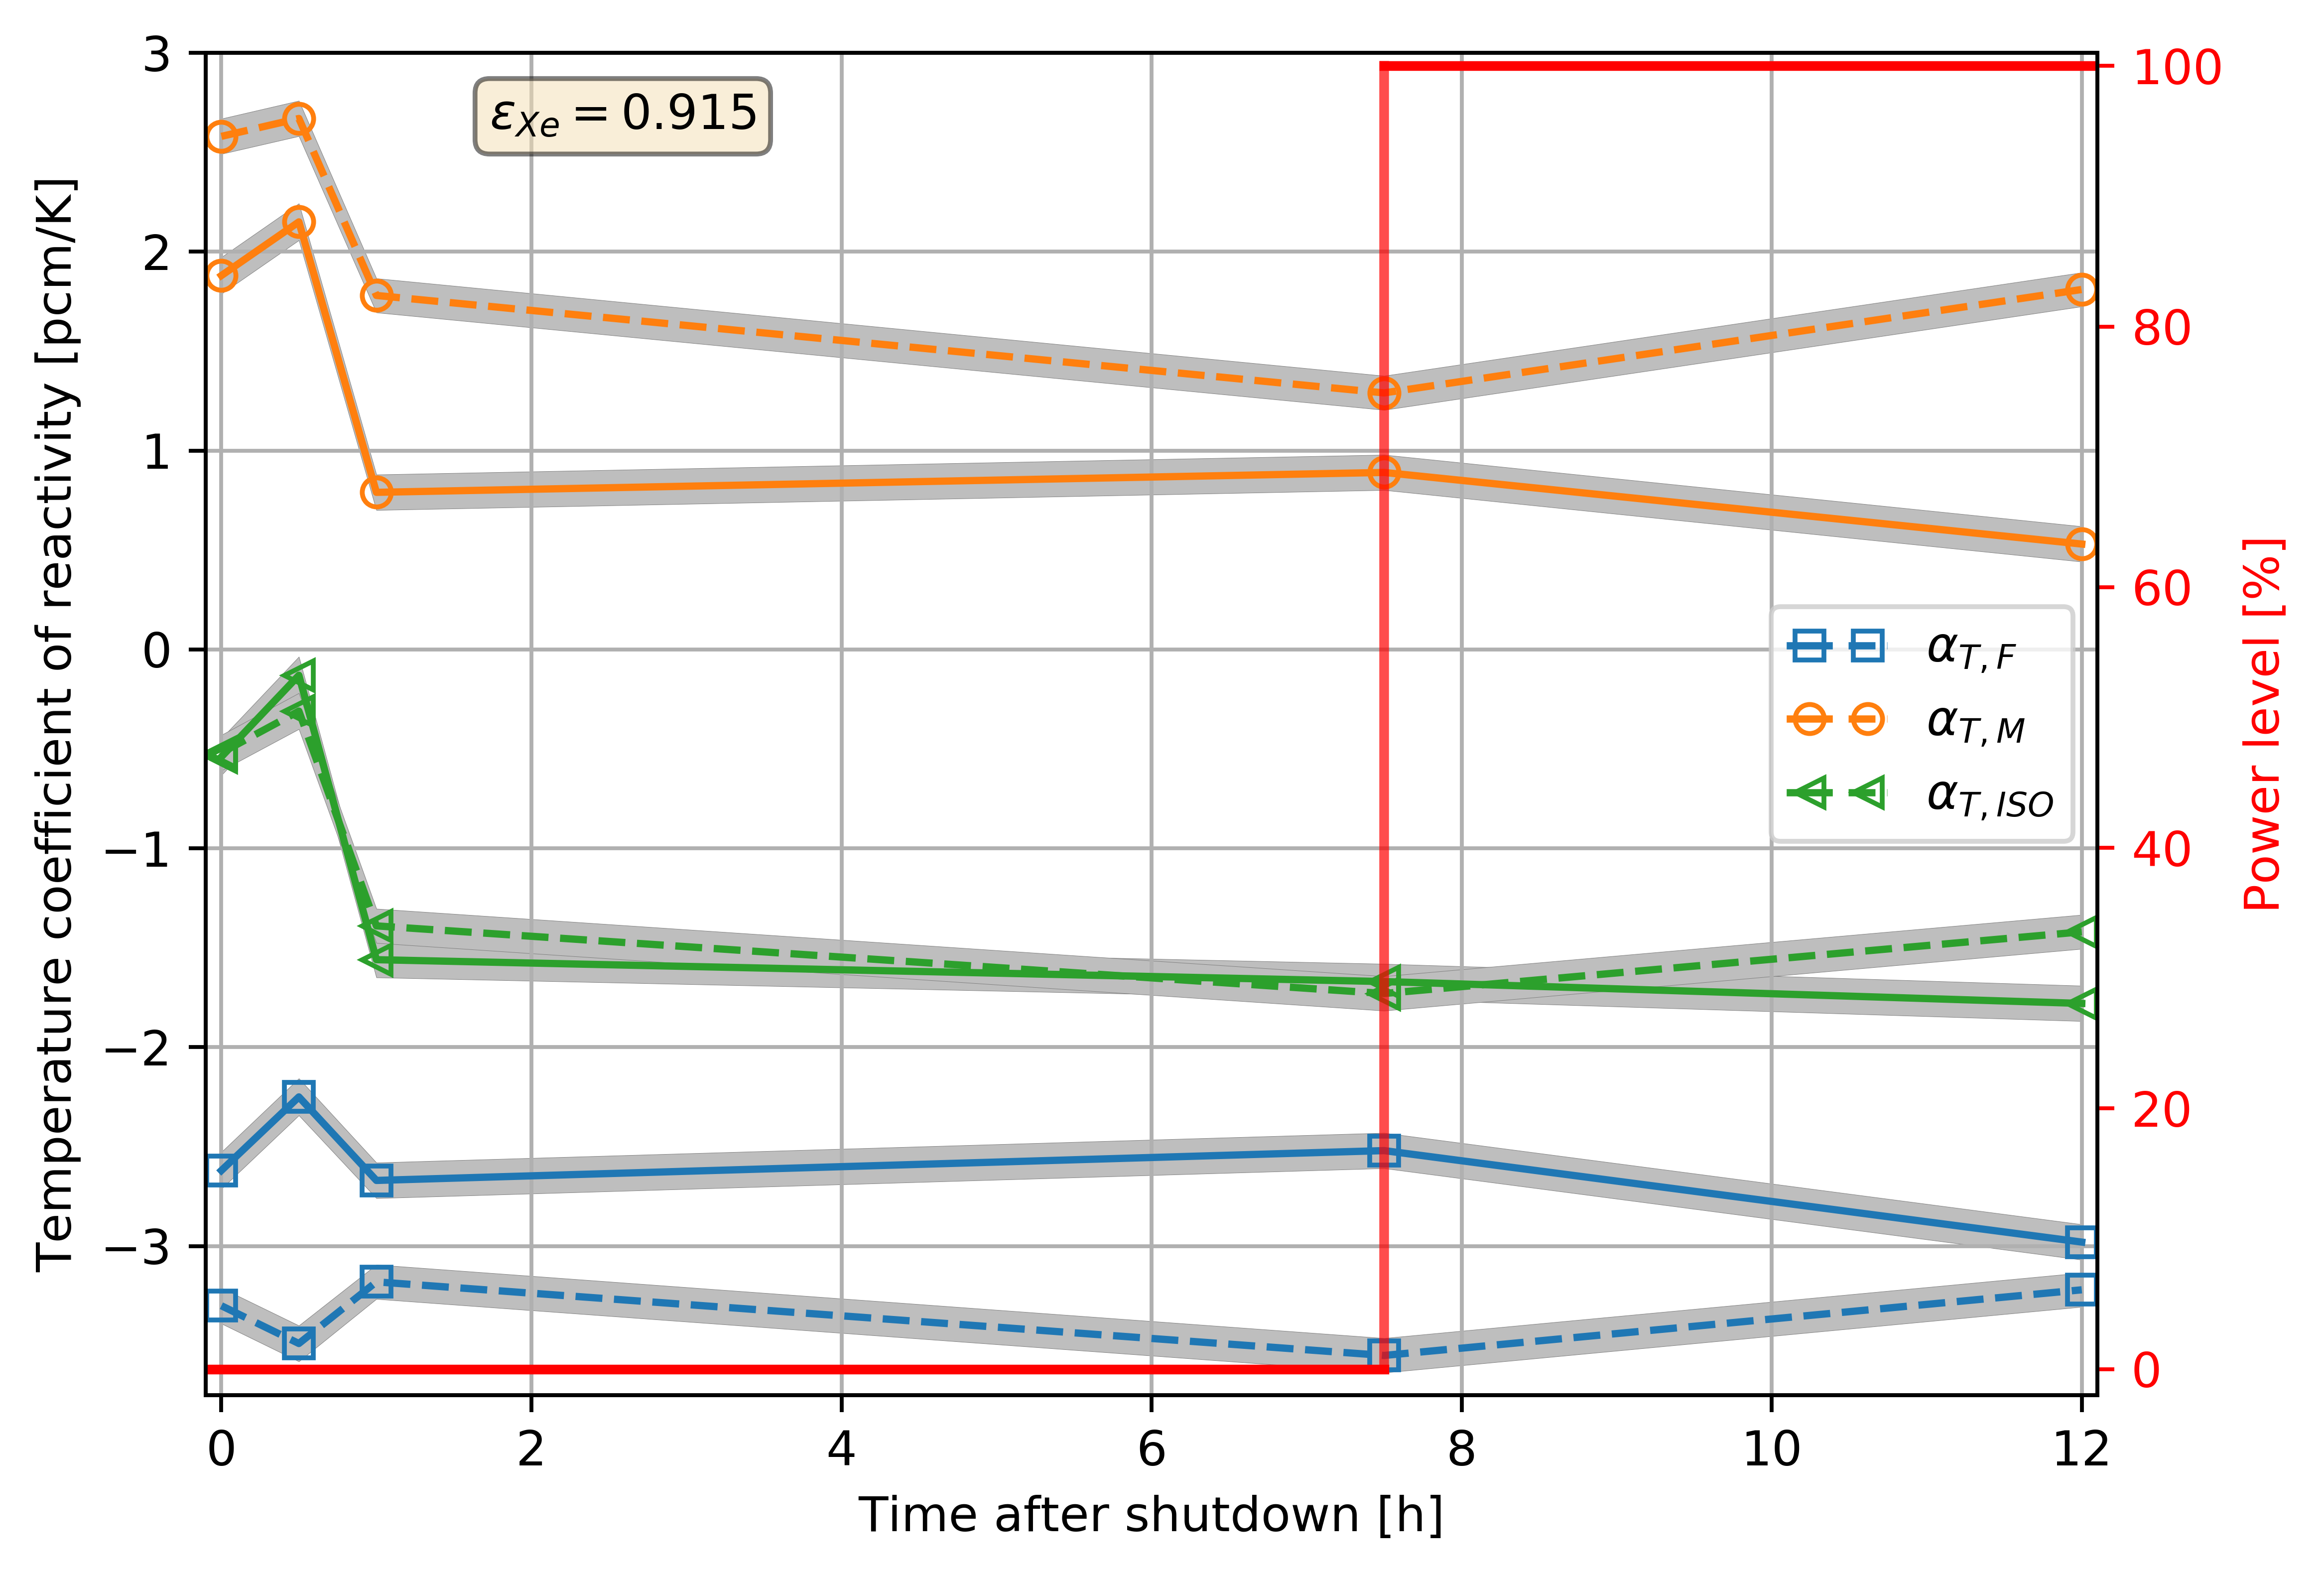
\includegraphics[width=0.95\textwidth]{ch6/saf_par/tc_evo_kl100.png}
	\vspace{-3mm}
	\caption{Temperature feedback coefficients during the postulated transient 
	for the \gls{MSBR} operating with moderate ($\epsilon_{Xe}=0.536$, upper) 
	and high ($\epsilon_{Xe}=0.915$, lower) gas removal efficiency at the 
	\gls{BOL} (dashed line) and after 30 years of operation (solid line).
	The	uncertainty, $\pm\sigma$, is shaded.}
	\label{fig:msbr-lf-tc-evo}
\end{figure}

The isothermal temperature coefficient, $\alpha_{ISO}$, is $-0.36\pm0.09$ 
$pcm/K$ at the beginning and remains stable during the first 30 minutes of the 
transient for the moderate removal efficiency case.  Then, as the gas removal 
system reduces $^{135}$Xe concentration in the core, $\alpha_{ISO}$ becomes 
even more negative: $-1.52\pm0.09$ $pcm/K$ when the $^{135}$Xe mass stabilized 
at 1.5 g in about 5 hours after the shutdown. After power ramp-up from 0\% to 
100\%, $\alpha_{ISO}$ also remains stable since the $^{135}$Xe mass increasing 
very slowly. On the whole, another exciting benefit from the online gas 
removal is improved passive safety (more powerful temperature feedback 
coefficient) throughout and, possibly, a few days after the postulated 
transient due to low concentration of the $^{135}$Xe in the fuel salt.

For the high gas removal efficiency regime ($\epsilon_{Xe}=0.915$), the 
isothermal temperature coefficient worsens from $-0.54\pm0.09$ $pcm/K$ to 
approximately $-0.22\pm0.09$ $pcm/K$ during first the 30 minutes after 
shutdown. 
Afterward, however, once the gas removal system extracted a significant 
fraction of the $^{135}$Xe from the fuel salt, $\alpha_{ISO}$ recovered, 
becoming significantly more 
negative ($-1.39$ and $-1.56$ $pcm/K$ at the \gls{BOL} and after 30 years of 
operation, respectively) due to the spectrum softening. In brief, \emph{the 
temperature feedback in the \gls{MSBR} becomes stronger when neutron poisons 
concentration in the fuel decreases}. As a result, flattening the $^{135}$Xe 
concentration curve improves the \gls{MSBR} passive safety.

Overall, the combination of fuel and moderator thermal feedback coefficients, 
$\alpha_{ISO}$, remains negative throughout the postulated transient. 
Moreover, a simpler and cheaper gas removal system with extraction 
efficiency $\epsilon_{Xe}=0.536$ provided more predictable thermal feedback 
coefficient dynamics throughout the transient due to 
a more gradual change in the $^{135}$Xe concentration.

\subsection{Void coefficient of reactivity}
Figure~\ref{fig:msbr-lf-void-evo} demonstrates the void coefficient of 
reactivity evolution during the postulated transient. 
In contrast with the \gls{TAP} \gls{MSR}, the void coefficient of reactivity 
after 30 years of full-power operation is substantially higher than at the 
startup for both gas removal regimes. The reason for this is the hardening of 
the \gls{MSBR} spectrum toward \gls{EOL}, which is the opposite of the 
\gls{TAP} \gls{MSR} spectrum evolution. Thus, an unexpected void insertion 
due, for example, to a gas separation system failure in the \gls{MSBR} would 
have more severe consequences for the \gls{EOL}. 
\begin{figure}[htbp!] % replace 't' with 'b' to 
	\centering
	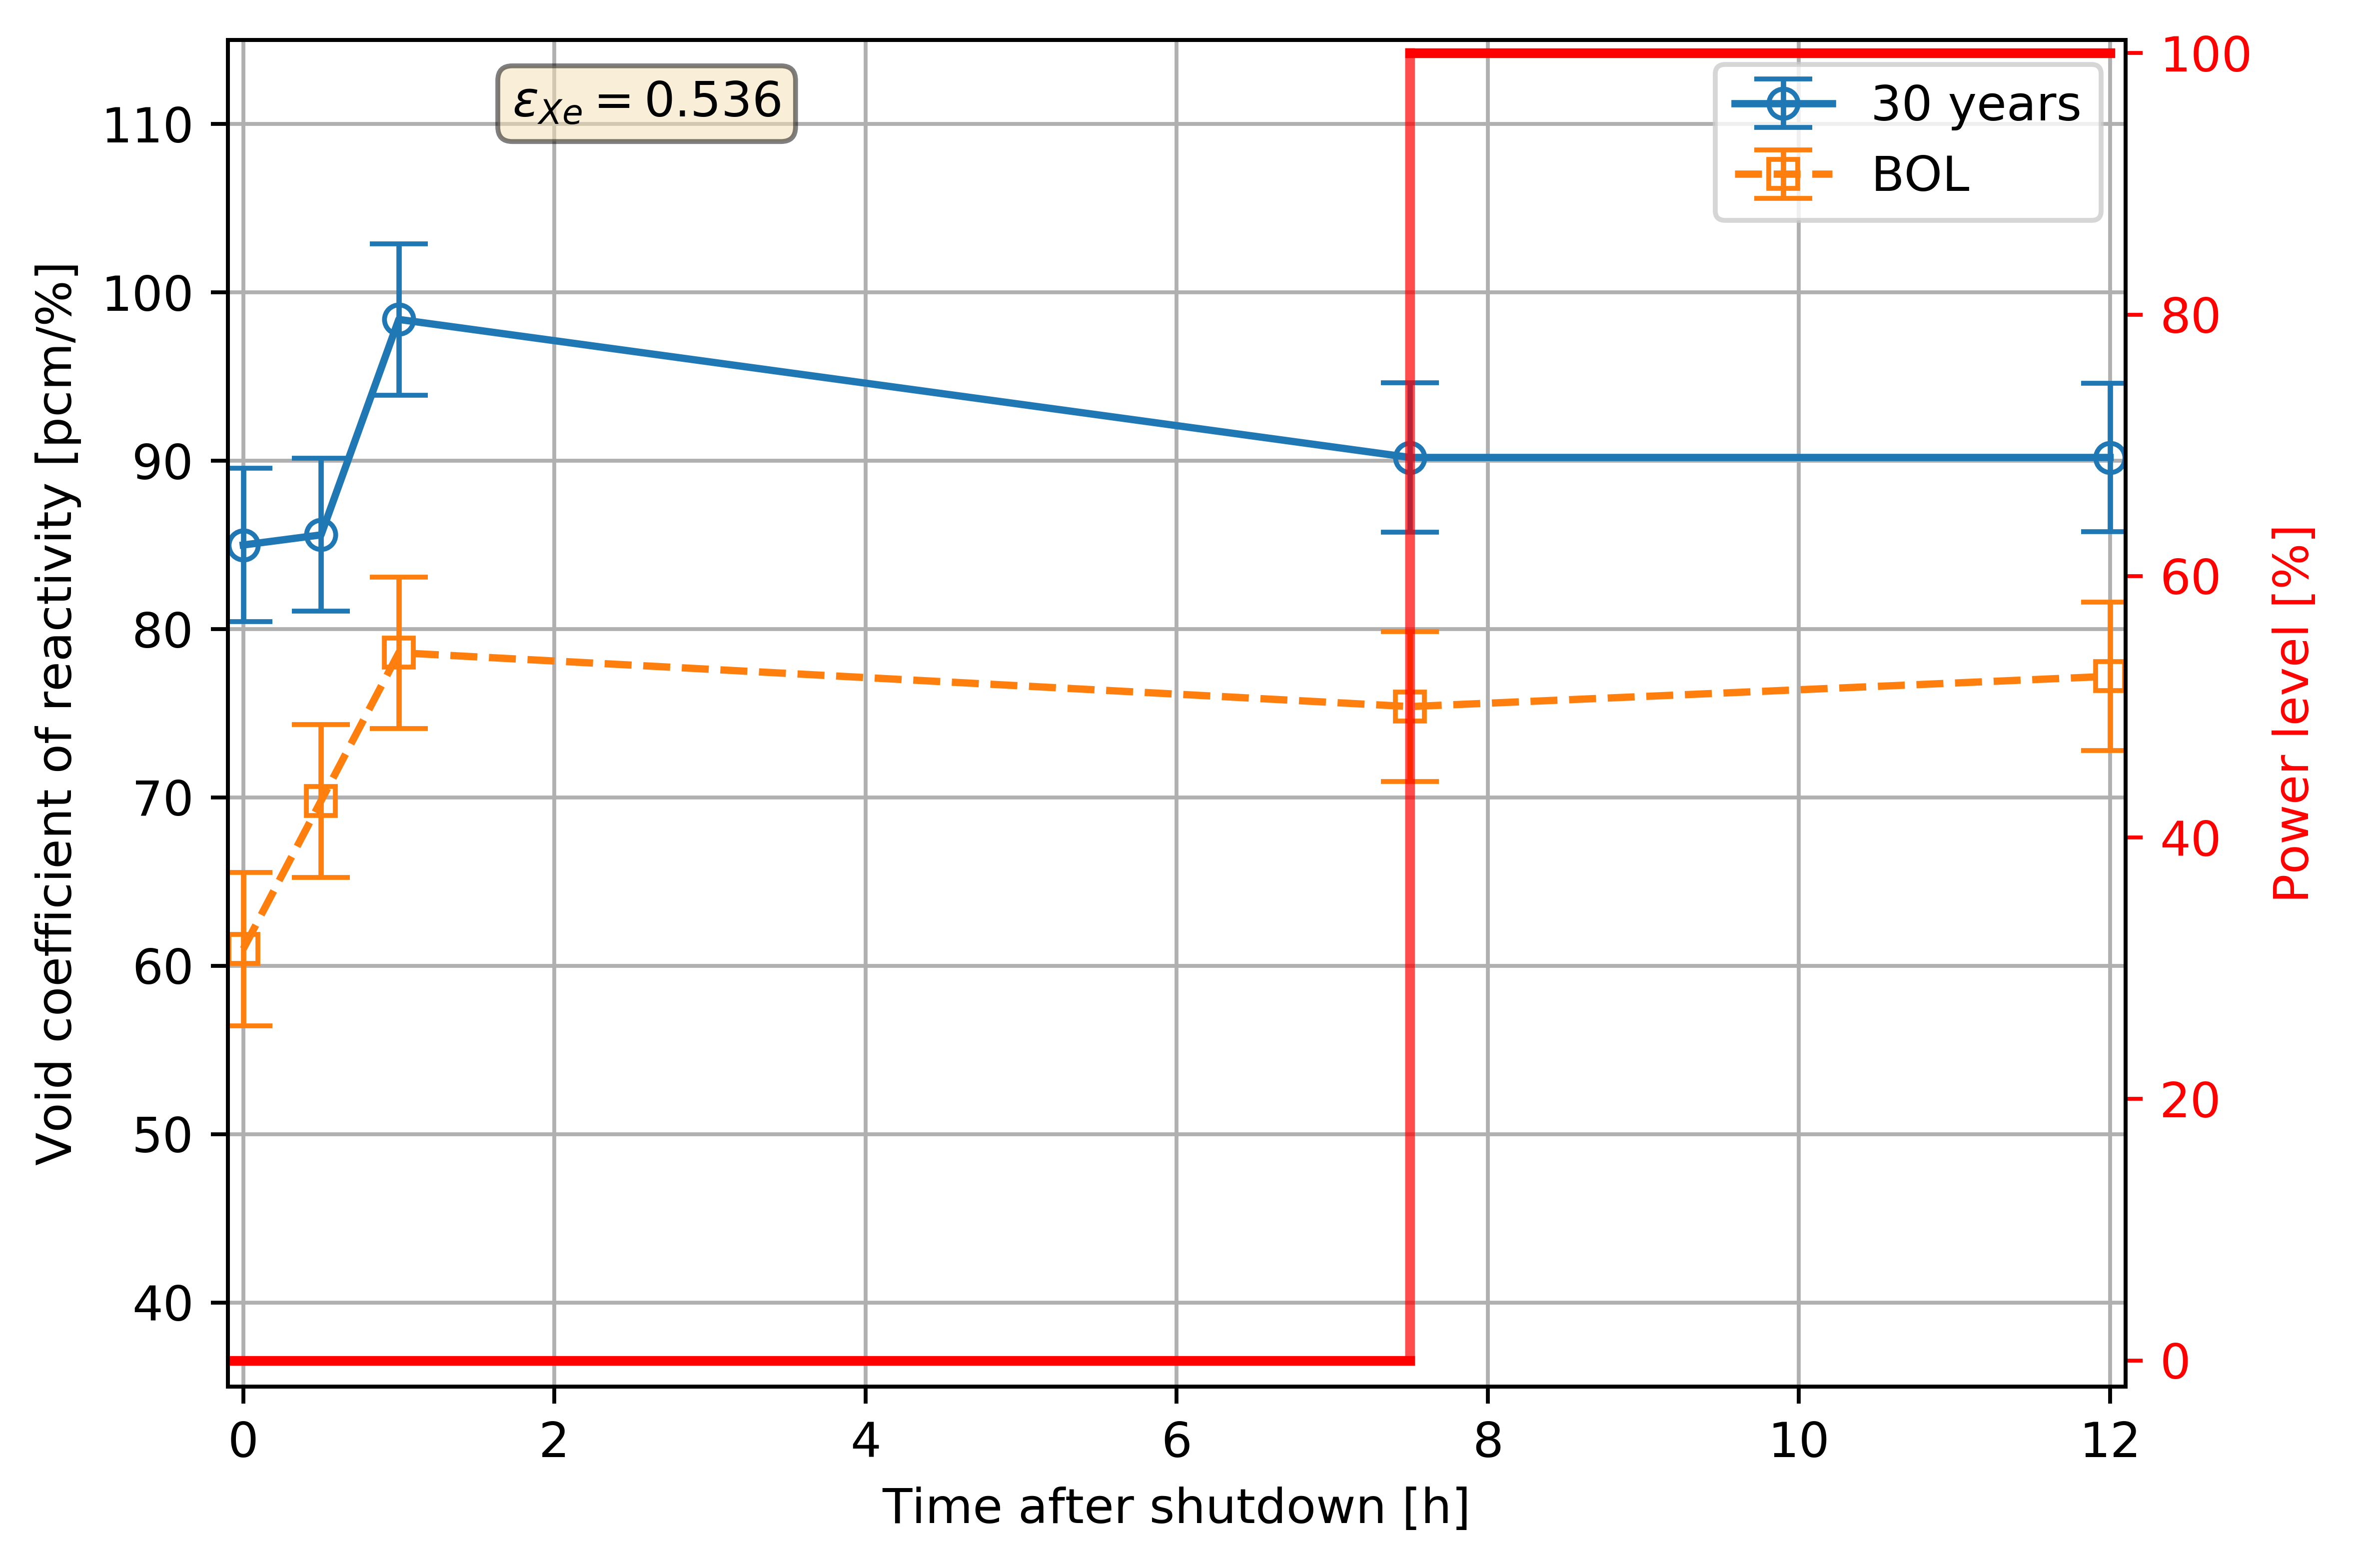
\includegraphics[width=0.92\textwidth]{ch6/saf_par/void_evo_kl25.png}\\
	\vspace{-12mm}
	\hspace{+0.05mm}
	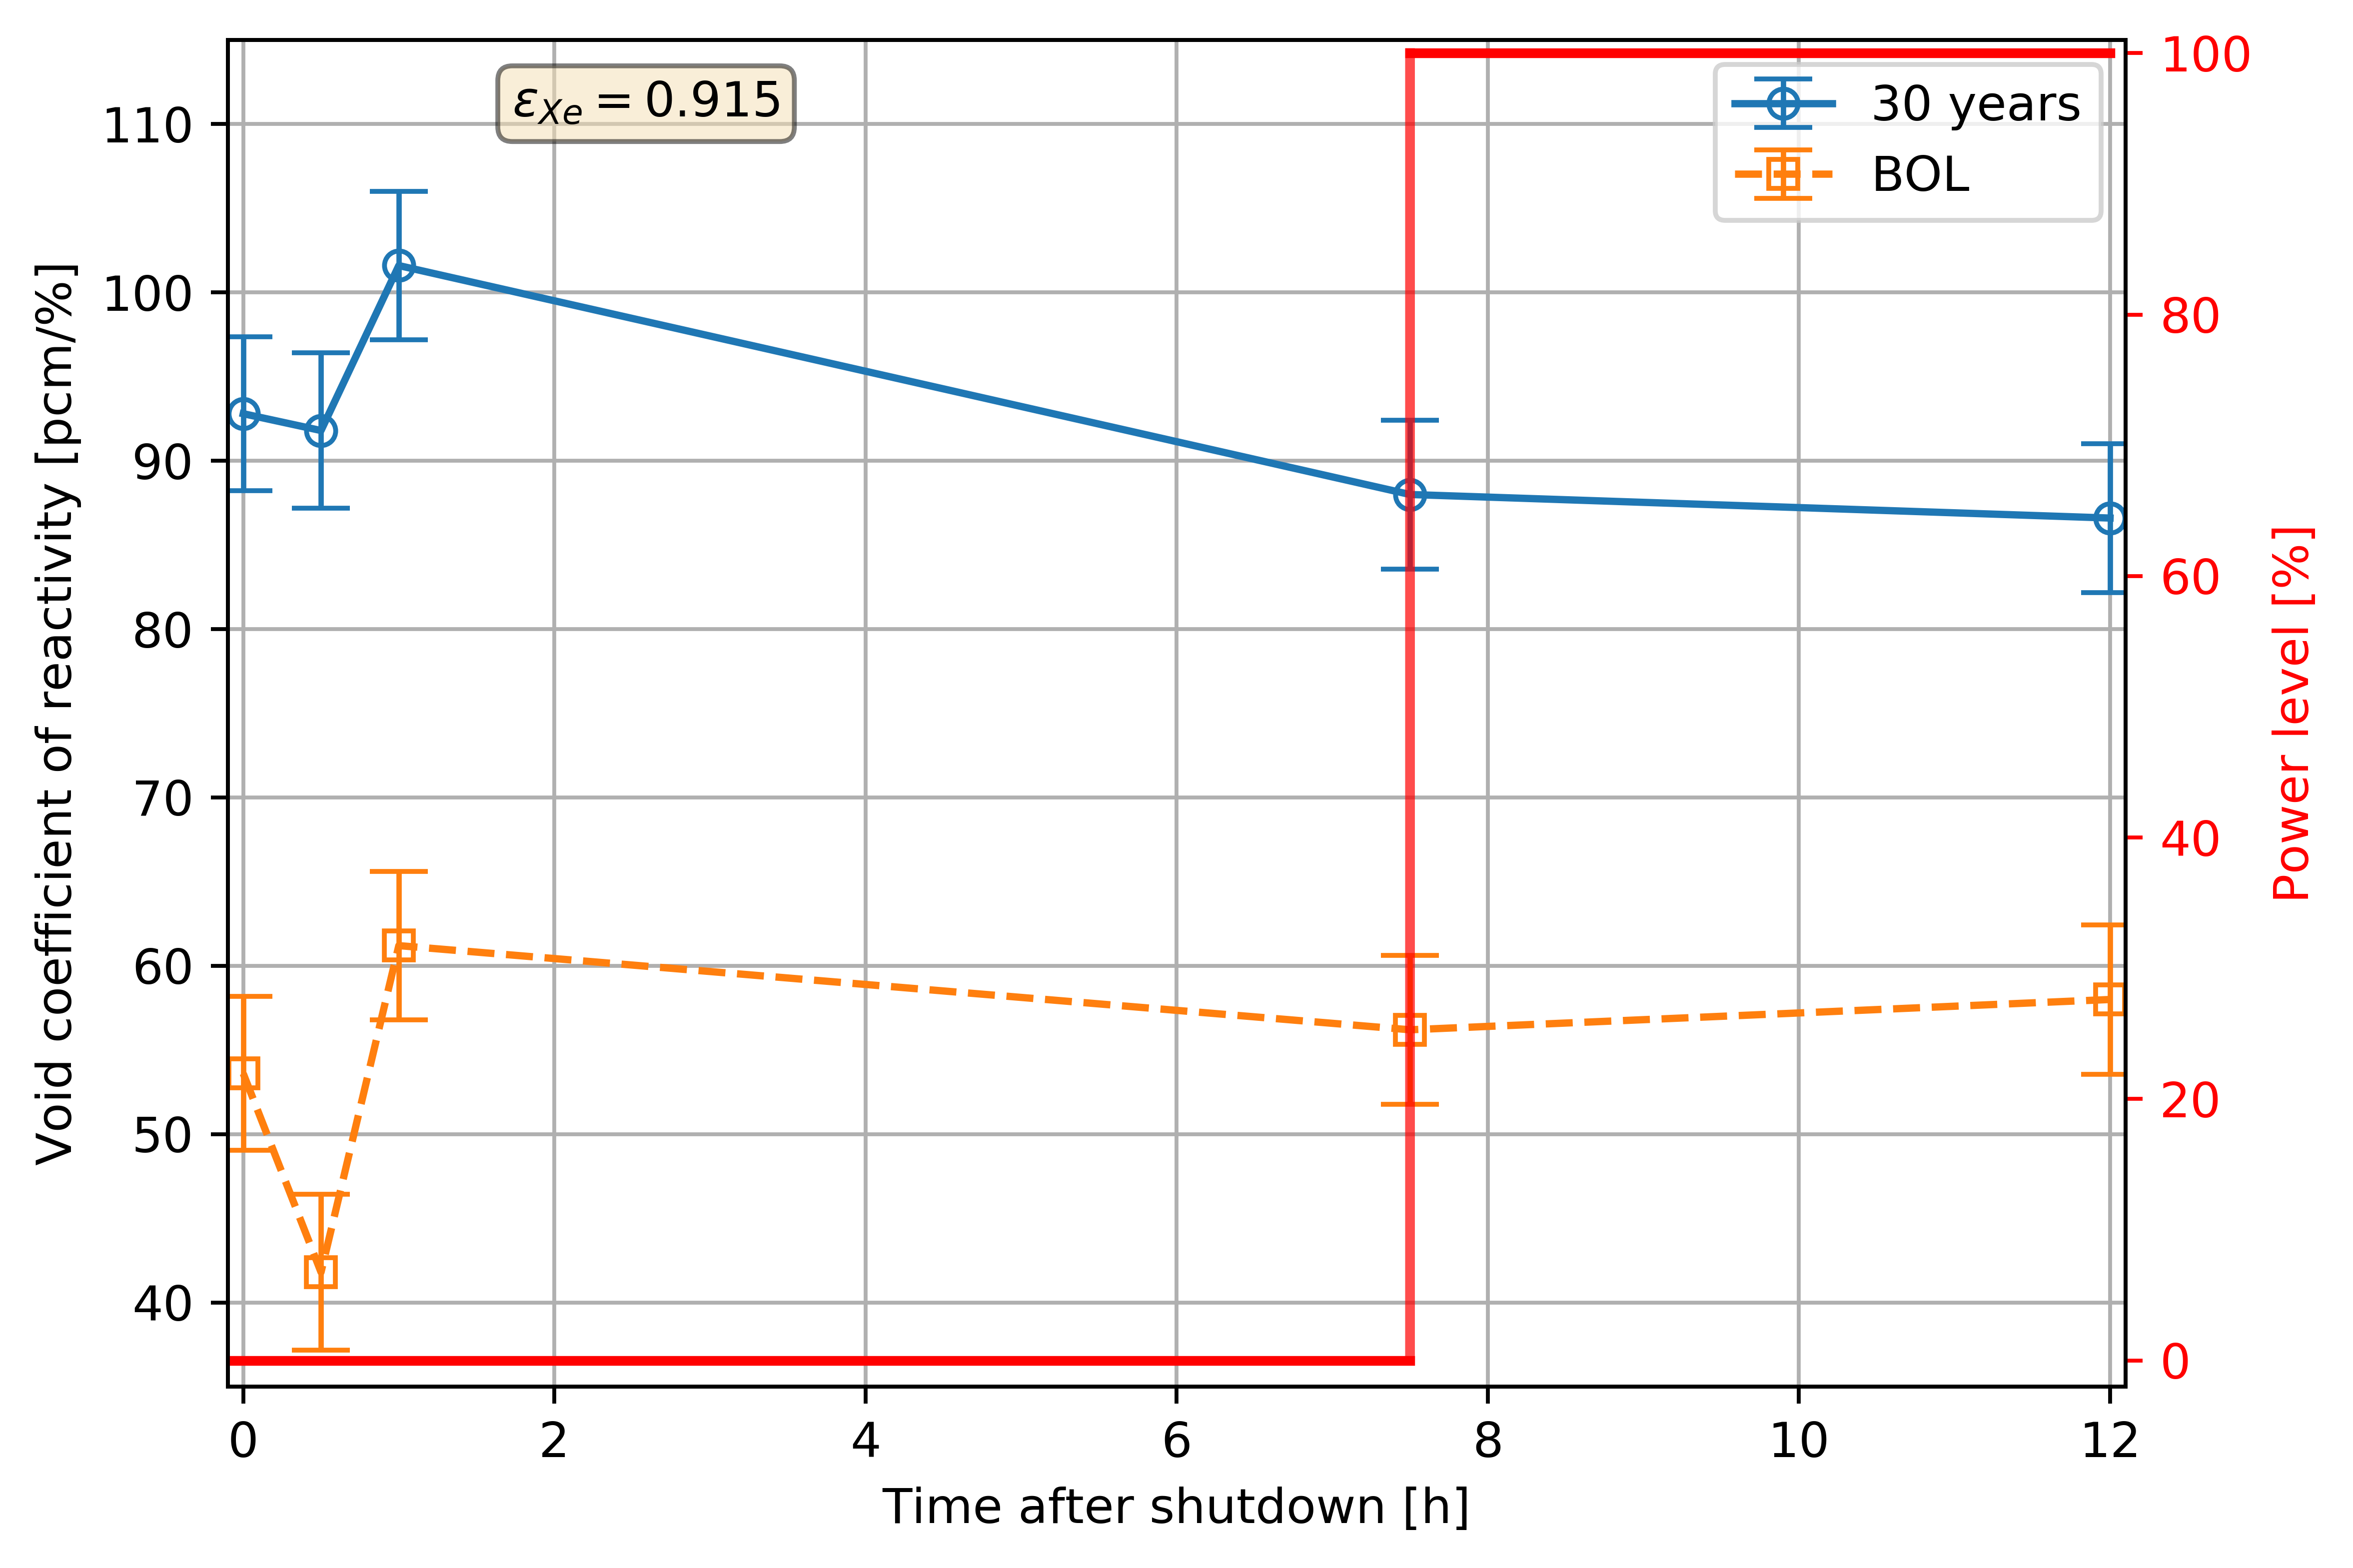
\includegraphics[width=0.92\textwidth]{ch6/saf_par/void_evo_kl100.png}
	\vspace{-3mm}
	\caption{Void coefficient of reactivity as a function of time during 
	postulated transient
for the \gls{MSBR} operating with moderate 
	($\epsilon_{Xe}=0.536$, upper) and high ($\epsilon_{Xe}=0.915$, lower) gas 
	removal efficiency at the \gls{BOL} (dashed line) and after 30 years of 
	operation (solid line).}
	\label{fig:msbr-lf-void-evo}
\end{figure}

For the high gas removal efficiency, $\alpha_V$ fluctuates during the 
postulated transient between 42 and 61 $pcm/$void\% at the \gls{BOL} and 
between 87 and 102 $pcm/$void\% after 30 years of operation. The $^{135}$Xe 
concentration spike caused corresponding $\alpha_V$ drop due to the short-term 
spectrum hardening. Then, $\alpha_V$ quickly recovers to its initial value. 
Similarly to the temperature feedback coefficient, the moderate gas removal 
efficiency provided more predictable $\alpha_V$ dynamics throughout the 
transient. Additionally, a small $\alpha_V$ fluctuation during 
the transient at the \gls{EOL} for the case with $\epsilon_{Xe}=0.536$ 
($\Delta\alpha_V\approx25$ $pcm/$void\%) would simplify the gas separator 
backup safety mechanism. 
Overall, all observed changes in the void coefficient of reactivity throughout 
the load-following transient for all cases are within the 3-$\sigma$ range 
($\sigma_{\alpha_V}\pm5$ $pcm/$\%). These observations should be taken 
into account in the \gls{MSBR} accident analysis and safety
justification.

\subsection{Reactivity control rod worth}
Figure~\ref{fig:lf-msbr-crw-evo} shows the control rod worth evolution 
during the postulated transient. For the high gas removal efficiency regime 
after 30 years of full-power operation, the control rod worth dropped by 
$46\pm9$ $pcm$ during the first 30 minutes after the shutdown. This happens 
due to a short-term spectrum hardening related to the $^{135}$Xe concentration 
peak. In the next 30 minutes, the CRW recovers to its initial value and keeps 
increasing throughout the transient because the gas removal system steadily 
reduces the $^{135}$Xe concentration in the core. Notably, the control rod 
worth is greater at the \gls{BOL} because the absorption cross section of 
$^{10}$B (used as an absorber in the control rods) declines rapidly with 
energy. Overall, the control rod worth benefits from the \gls{MSBR} spectrum 
softening toward \gls{EOL}.

For the moderate gas separation efficiency regime, the control rod worth 
remains almost constant during the first hour after shutdown. Afterward, the 
CRW increased by 4\% due to the spectrum softening caused by the increased 
$^{135}$Xe concentration. As for other safety parameters, the control rod 
worth also benefits from a less effective gas removal system due to smother 
xenon concentration dynamics and a more predictable neutron spectrum shift. 
\begin{figure}[htbp!] % replace 't' with 'b' to 
	\centering
	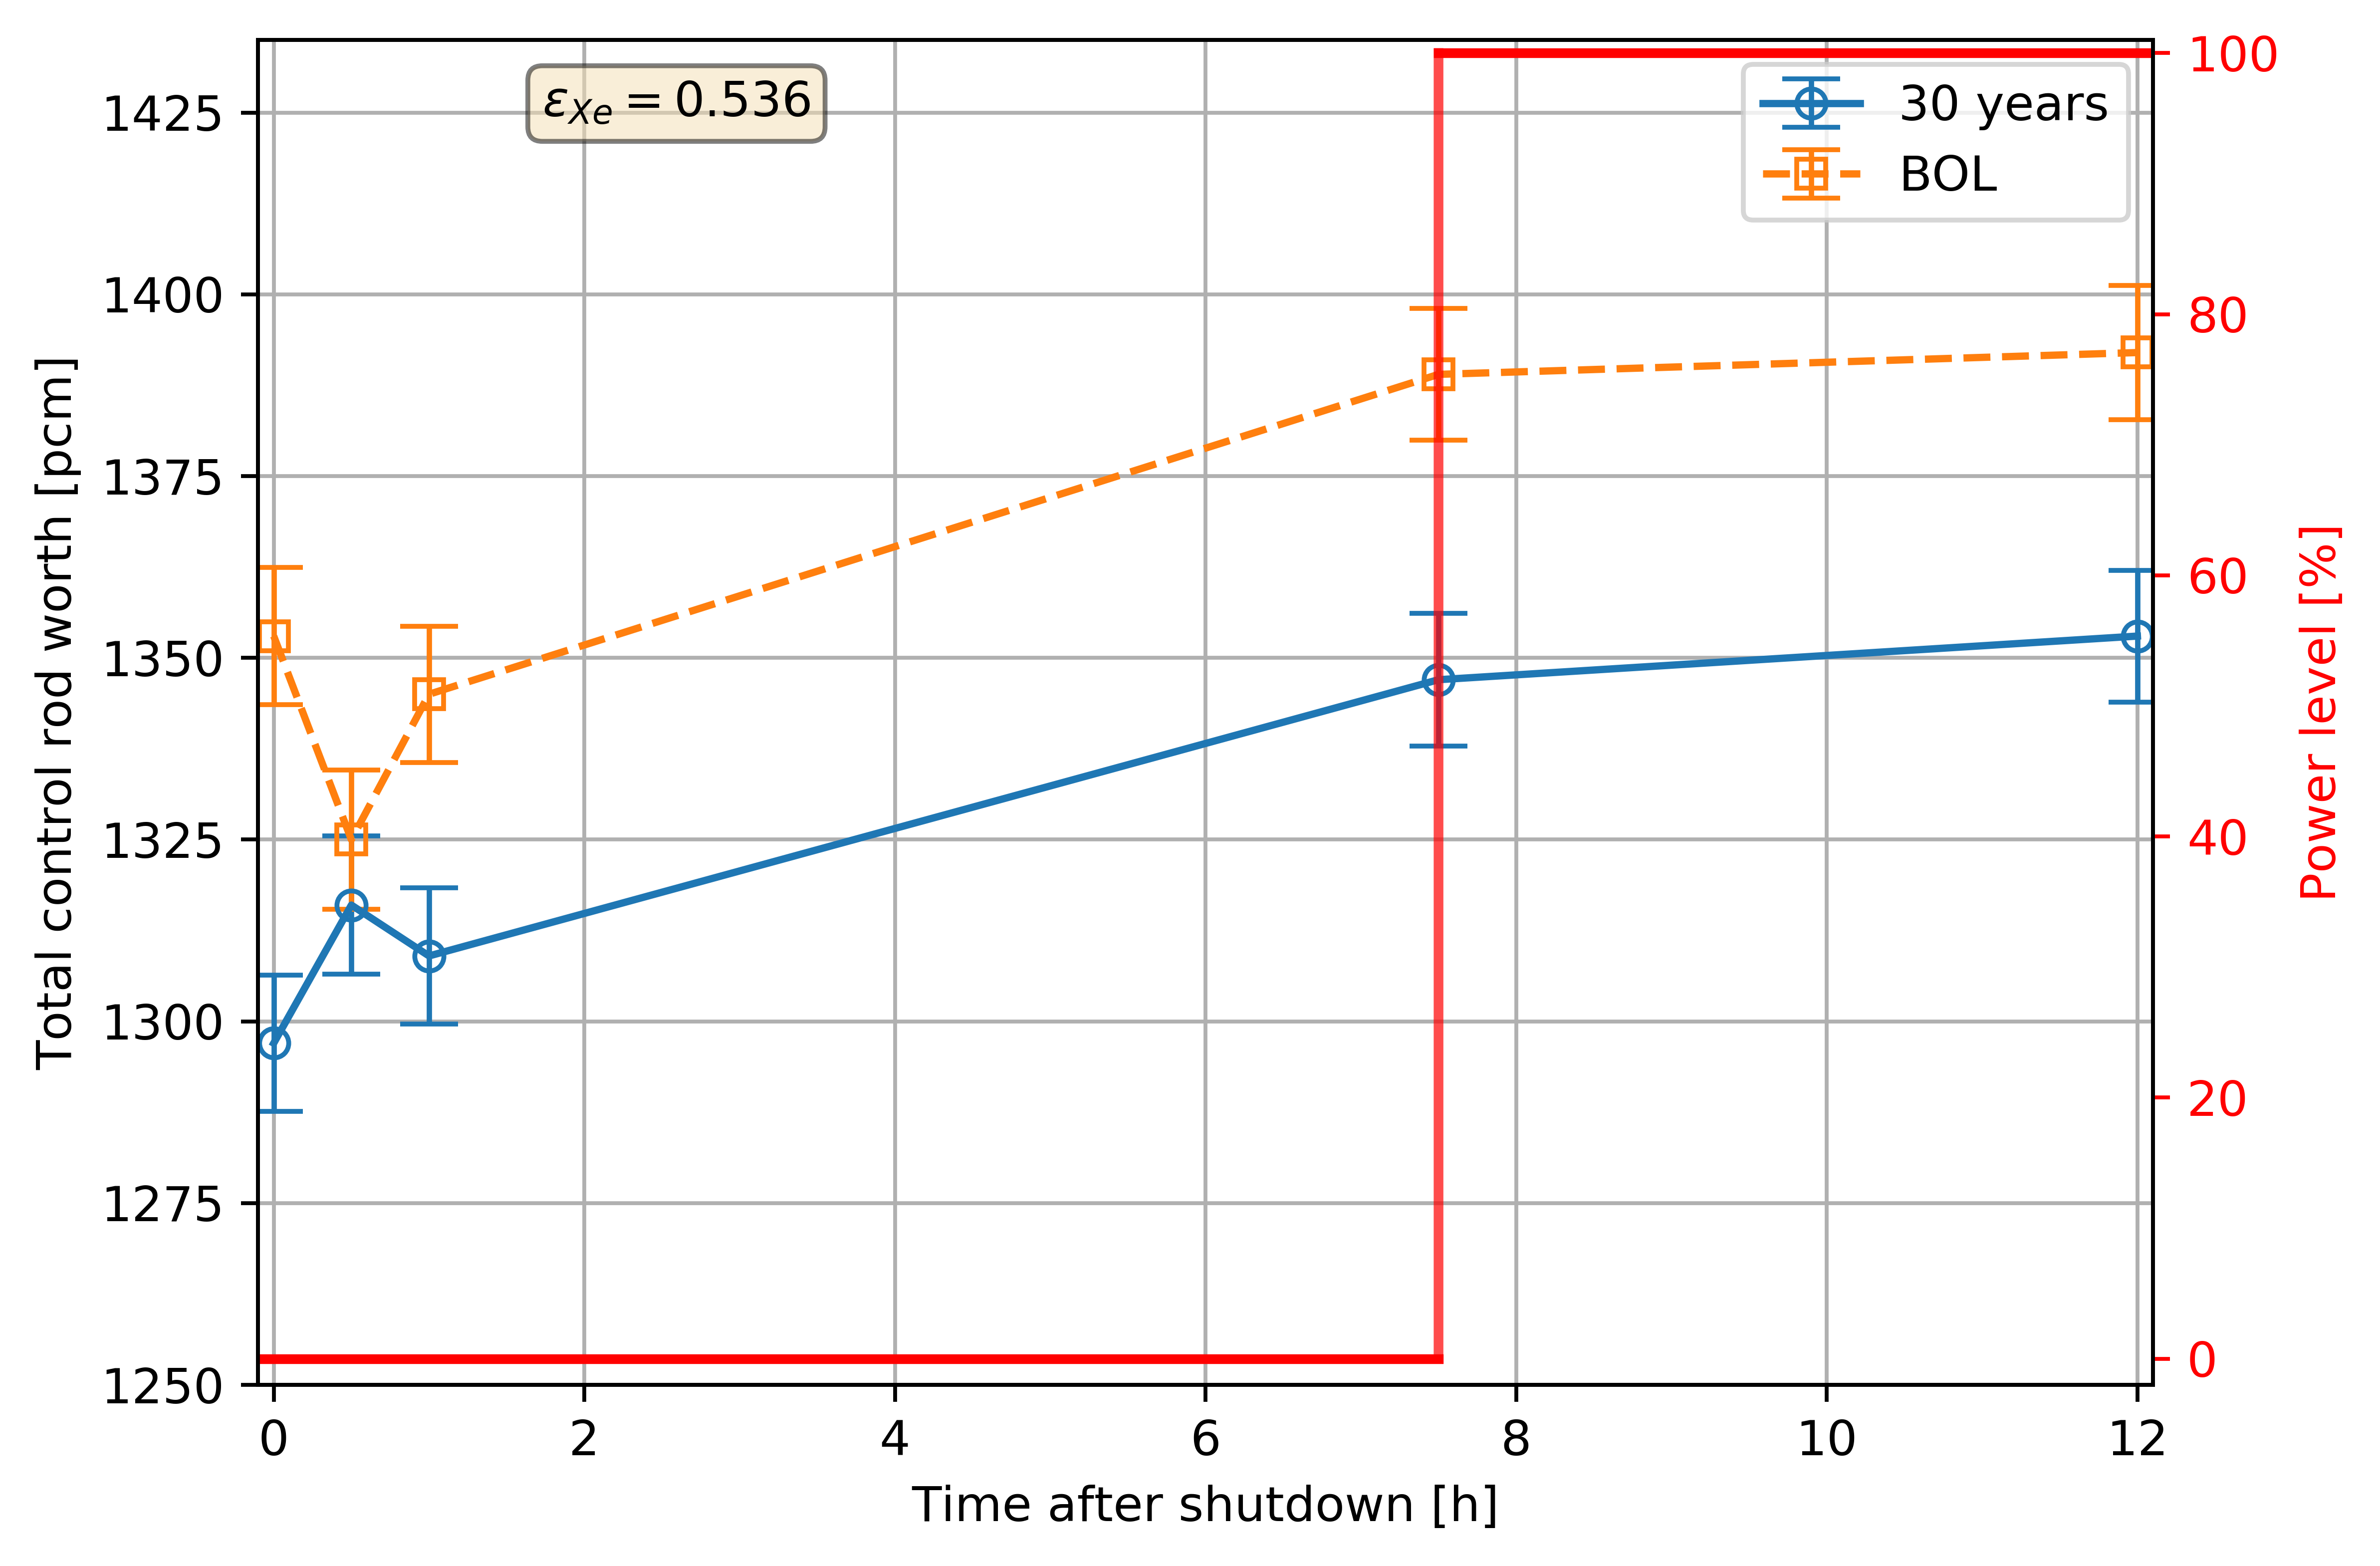
\includegraphics[width=0.95\textwidth]{ch6/saf_par/crw_evo_kl25.png}\\
	\vspace{-10mm}
	\hspace{+0.05mm}
	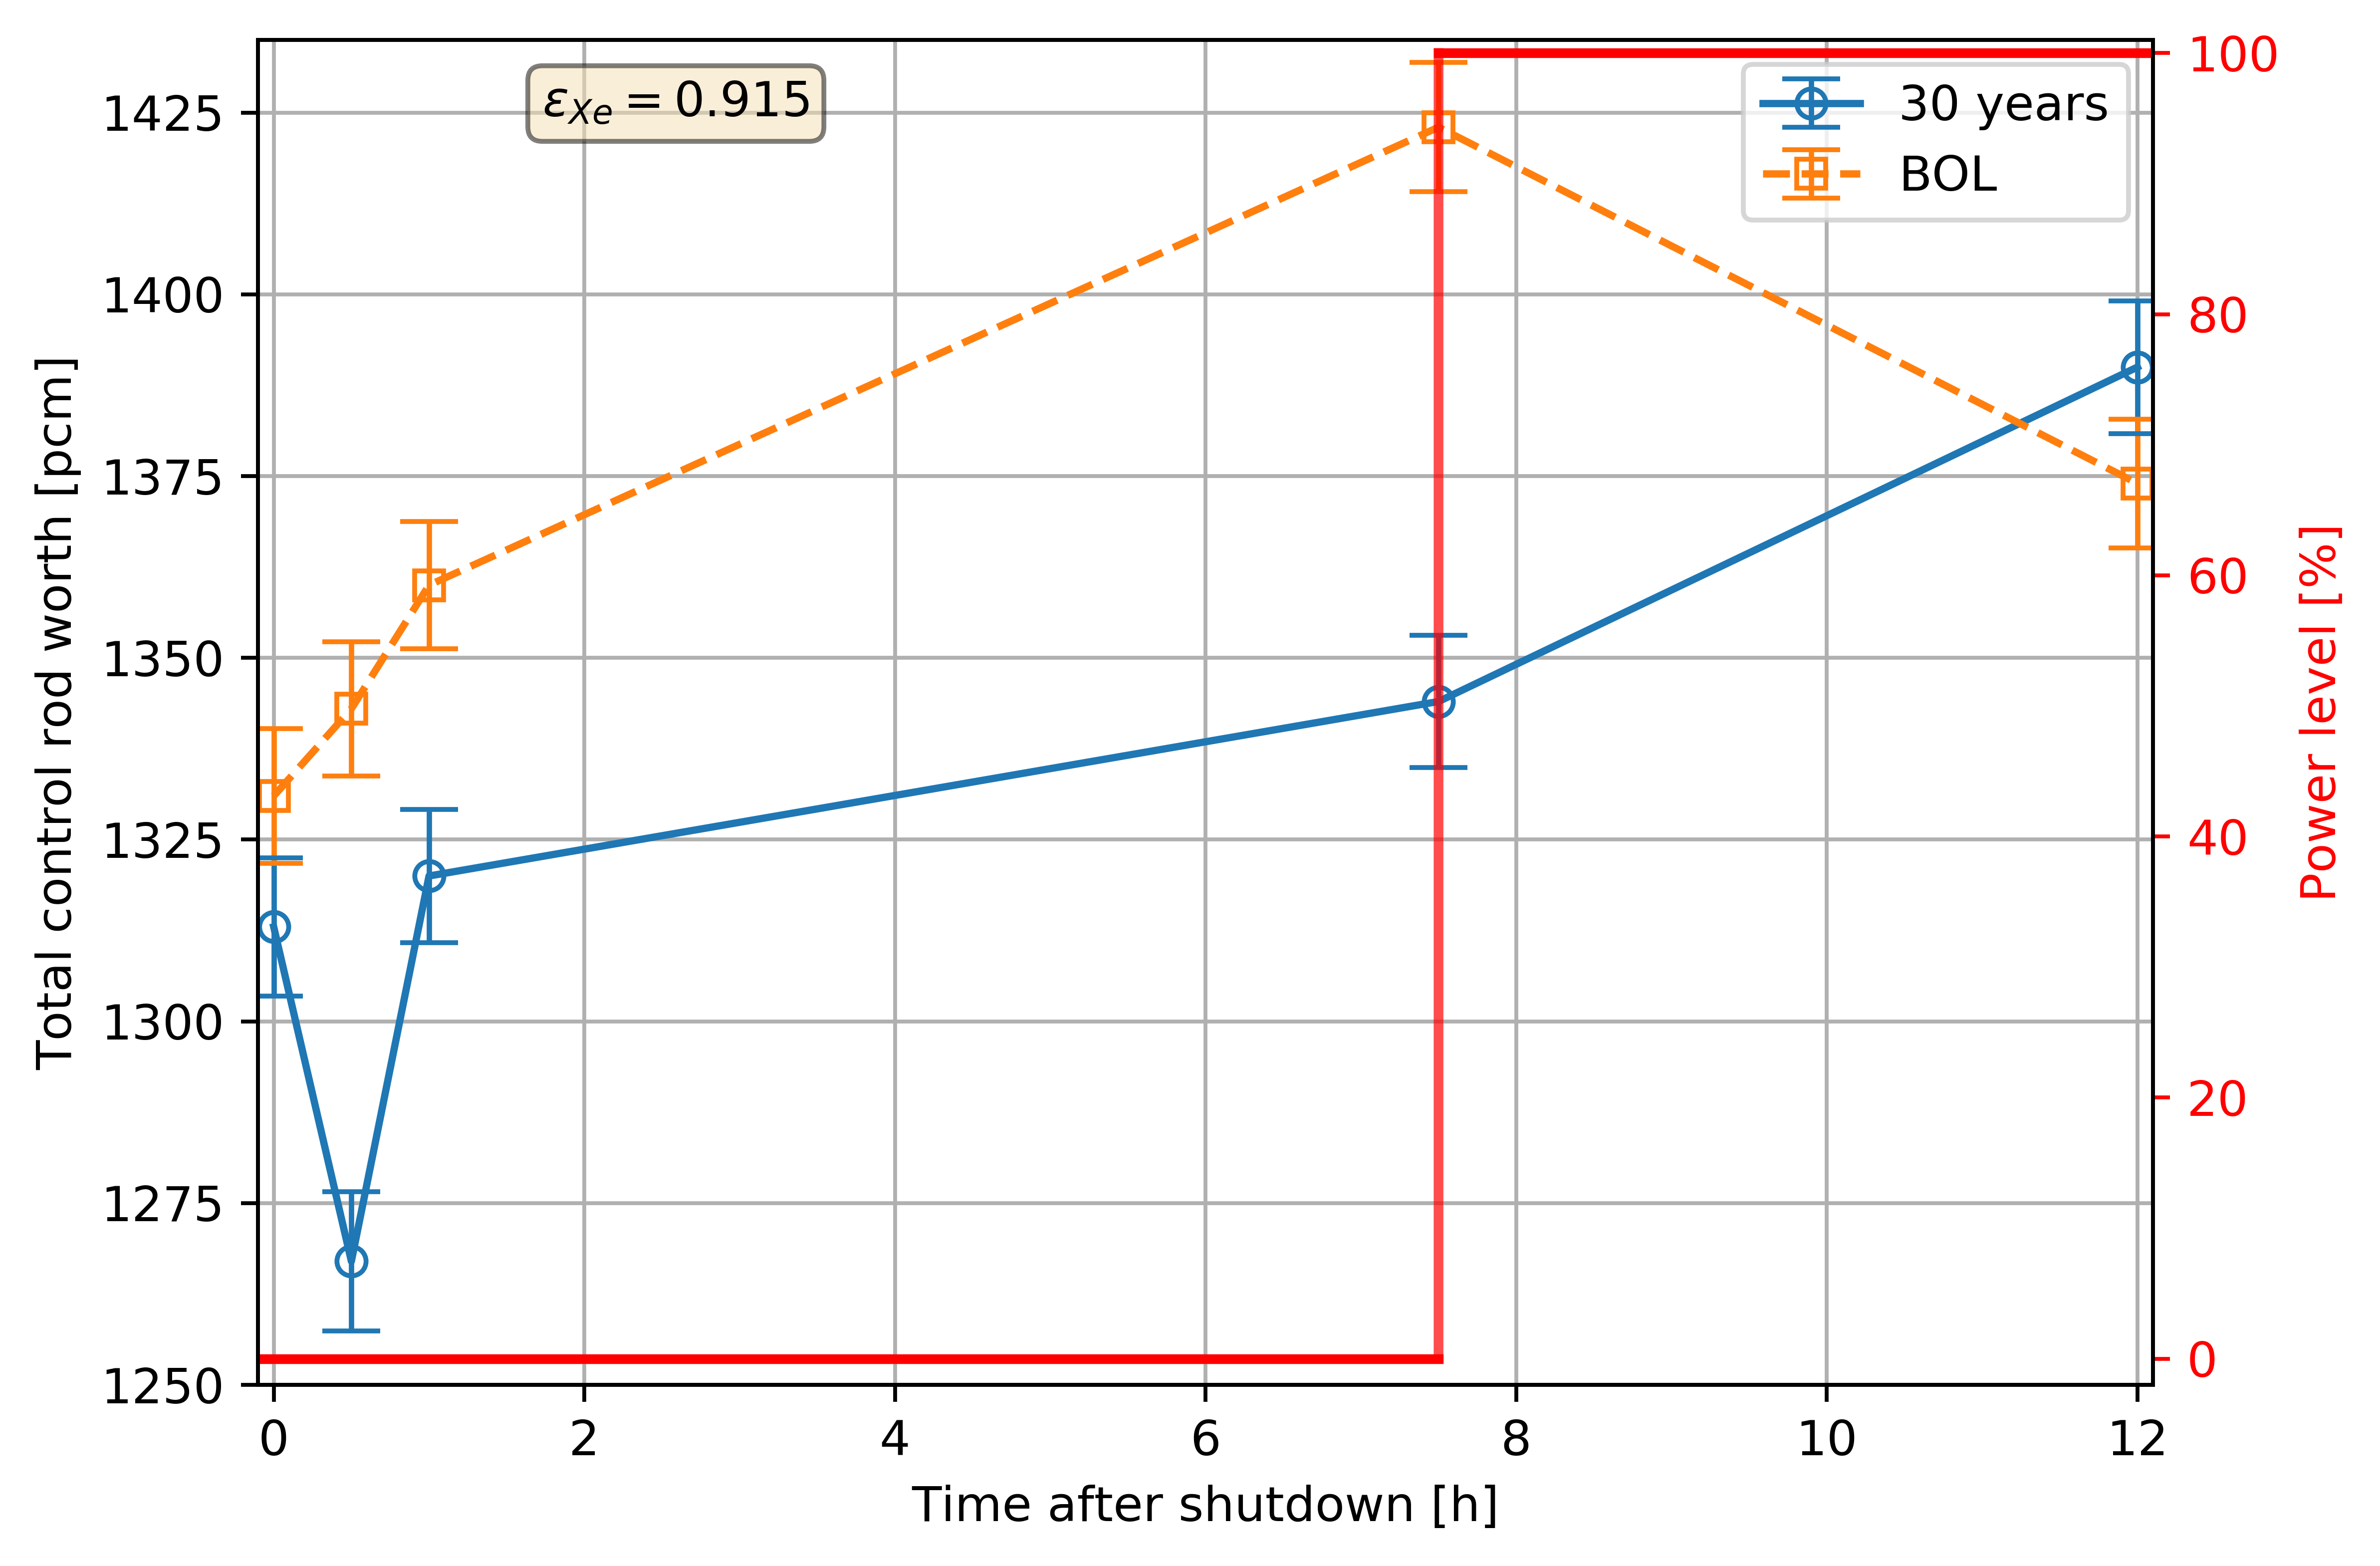
\includegraphics[width=0.95\textwidth]{ch6/saf_par/crw_evo_kl100.png}
	\vspace{-3mm}
	\caption{Total control rod worth as a function of time during 
		postulated transient
for the \gls{MSBR} operating with moderate 
		($\epsilon_{Xe}=0.536$, upper) and high ($\epsilon_{Xe}=0.915$, lower) 
		gas removal efficiency at the \gls{BOL} (dashed line) and after 30 
		years of operation (solid line).}
	\label{fig:lf-msbr-crw-evo}
\end{figure}

Unfortunately, the total control rod worth is insufficient to shut down the 
reactor throughout the postulated transient for both medium and high removal 
efficiency ($\epsilon_{Xe}=0.536$ and $\epsilon_{Xe}=0.915$). The reactivity 
change during the 
transient is up to 2600 $pcm$, while the total control rod worth is only about 
$1250-1425$ $pcm$. The \gls{MSBR} was designed with only two graphite and two 
boron-carbide rods located in the center of the core (see 
Figure~\ref{fig:msbr_elev_view}) for operative reactivity control and relied 
heavily on fissile feed adjustment as a primary reactivity control 
mechanism. However, the fissile feed cannot be adjusted quickly, and nuclear  
regulations require control rods to have sufficient worth to shut down the 
reactor safely at any time. Therefore, the control rod design in the 
\gls{MSBR} must be reexamined to ensure the total control rod worth of at 
least 3000 $pcm$ to ensure safety during the transient with rapid power change.


\section{Concluding remarks}
This chapter demonstrated SaltProc v1.0 capabilities to simulate the 
short-term depletion with the power variation from 0\% to 100\% for the 
\gls{MSBR}. I applied methodology from Chapter 5 to investigate the xenon 
poisoning effect in the \gls{MSBR} for three various gas removal system 
regimes: (1) no gas removal, (2) moderate gas removal efficiency, and (3) high 
gas removal efficiency. 

When the gas removal system is inactive, the $^{135}$Xe concentration peaked 
in about 7.5 hours after shutdown, which caused the reactivity drop by 1457 
and 1035 $pcm$ for the startup and equilibrium fuel salt composition. Such a
negative effect of the xenon poisoning is consistent with other thermal 
reactor designs (i.e., -1500 $pcm$ for \gls{PWR} 
\cite{rykhlevskii_impact_2019}). In contrast with results for the \gls{TAP} 
\gls{MSR} in Chapter 5, the \gls{MSBR} demonstrated a significant negative 
impact of the $^{135}$Xe concentration spike on the core neutronics after 
shutdown. The reason for that is significantly greater initial 
$^{135}$I/$^{135}$Xe concentration ratio: 2.45 and 1.0 for the \gls{MSBR} and 
\gls{TAP} reactor at the \gls{BOL}, respectively. Thus, the $^{135}$Xe peak is 
significantly higher for the \gls{MSBR} than for the \gls{TAP} reactor: +56\% 
and +0.33\%, respectively. Finally, the $^{135}$Xe parasitically absorbs 
substantially more neutrons in the thermal (\gls{MSBR}) than in the epithermal 
(\gls{TAP} \gls{MSR}) neutron spectrum, which amplifies the xenon poisoning 
effect when the spectrum softens. In contrast with the spectrum thermalization 
toward \gls{EOL} in the \gls{TAP} reactor, in the \gls{MSBR}, the neutron 
spectrum hardens toward \gls{EOL} due to plutonium and other strong absorbers 
accumulation in the fuel salt. Thus, for the \gls{MSBR}, the xenon poisoning 
effect becomes less severe toward \gls{EOL}. 

The online gas removal in the \gls{MSBR} demonstrated an impressive positive 
impact on the core neutronics. The gas removal system operation almost 
eliminated the effect of xenon poisoning by removing the vast majority of 
$^{135}$Xe during the first hour after the shutdown. During the first 
30-minute interval, 
the reactivity dropped by 161 and 189 $pcm$ for moderate and high removal 
efficiency, respectively. Afterward, the reactivity raised by 
$2700$ $pcm$ for both efficiencies in a few hours because the $^{135}$Xe 
inventory fell from 14 to 1-2 g. Indeed, the $^{135}$Xe loss due to decay 
and active gas removal significantly  overcame its gain from the $^{135}$I 
decay only (no fission happens; thus, no new $^{135}$I is produced). Notably, 
the amplitude of the reactivity swing after shutdown is more significant for 
the \gls{BOL} when the xenon reactivity worth is greater due to the softer 
neutron spectrum. Finally, significantly lower gas removal efficiency 
($\epsilon_{Xe}=0.536$ instead of 0.915) provided comparable benefits to the 
\gls{MSBR} core neutronics during the postulated load-following transient.

Finally, this chapter demonstrated that the \gls{MSBR} maintains necessary 
safety margins throughout the postulated load-following transient. Thus, the 
temperature coefficient of reactivity and the total control rod worth worsen 
slightly during the first 30 minutes of the transient when the $^{135}$Xe 
concentration peaked, causing corresponding neutron spectrum hardening. After 
that, the fast $^{135}$Xe concentration decline improved all safety and 
operational parameters among the cases. Unfortunately, the reactivity worth of 
two control rods made of boron carbide (B$_4$C) is insufficient to compensate 
for huge reactivity change after the shutdown. Even though the total control 
worth rises throughout the transient, the reactivity system design is 
unfeasible for load-following and must be redesigned. 

In conclusion, the xenon poisoning impact on the core neutronics is much 
stronger in the \gls{MSBR} than in the \gls{TAP} \gls{MSR}. Thus, the 
\gls{MSBR} without gas removal is incapable of flexible restart after
reducing power from 100\% to 0\%. However, online gas removal, even with 
moderate separation efficiency, helps eliminate the iodine pit problem and 
enable the load-following capability of the \gls{MSBR} without compromising 
its safety. Another benefit from the online gas removal is a stronger thermal 
feedback.

The work determined that the gas removal system should have a smart control 
coupled with reactivity control and power regulation systems.
Such a system must boost the separation efficiency right before and during the 
first few minutes after power drop to flatten the $^{135}$Xe peak. 
Then, the control system should reduce the removal efficiency to avoid a
sizeable positive reactivity insertion due to a fast $^{135}$Xe concentration 
drop. Finally, a more detailed study of power-changing transients must be 
performed using SaltProc v1.0 with better time resolution (i.e., a 1-min 
interval) to understand better how to adjust the gas removal efficiency during 
power adjustments.
